\documentclass[11pt,a4paper]{article}

% ---------------------------------------------------------------------------
% Reliable repeated harvesting in a finite-molecule autocatalytic reactor:
% a source-level finite-horizon operating theorem with a machine-checked proof.
%
% Author metadata: set the macros below before submission.  They are
% deliberately left blank in this version.  \CompanionAuthor is the author
% printed for the companion manuscripts in refs.bib; \RepositoryNote is where
% the public repository location goes.
% ---------------------------------------------------------------------------
\newcommand{\PaperAuthor}{}
\newcommand{\PaperAffiliation}{}
\newcommand{\PaperDate}{15 September 2026}
\newcommand{\CompanionAuthor}{Anonymous}
\newcommand{\RepositoryNote}{The repository location will be supplied with the author information.}

\usepackage[T1]{fontenc}
\usepackage[utf8]{inputenc}
\usepackage{lmodern}
\usepackage{microtype}
\usepackage[a4paper,margin=1.05in]{geometry}
\usepackage{amsmath,amssymb,amsthm,mathtools}
\usepackage{booktabs}
\usepackage{array}
\usepackage{longtable}
\usepackage{enumitem}
\usepackage{xcolor}
\usepackage{graphicx}
\usepackage{tikz}
\usetikzlibrary{arrows.meta,positioning,calc}
\usepackage[obeyspaces,spaces]{url}
\usepackage[numbers,sort&compress]{natbib}
\usepackage[colorlinks=true,linkcolor=blue!55!black,citecolor=blue!55!black,urlcolor=blue!55!black]{hyperref}
\hypersetup{pdftitle={Reliable repeated harvesting in a finite-molecule autocatalytic reactor},
  pdfkeywords={autocatalysis, stochastic reaction networks, serial transfer, finite-copy reliability, uniformization, exponential martingales, template replication, Lean}}

\DeclareUrlCommand\lean{\urlstyle{tt}}
\setlist{itemsep=2pt,topsep=3pt}
\setlength{\emergencystretch}{1.5em}
\graphicspath{{figures/}}

\theoremstyle{plain}
\newtheorem{theorem}{Theorem}[section]
\newtheorem{proposition}[theorem]{Proposition}
\newtheorem{lemma}[theorem]{Lemma}
\newtheorem{corollary}[theorem]{Corollary}
\theoremstyle{definition}
\newtheorem{definition}[theorem]{Definition}
\theoremstyle{remark}
\newtheorem{remark}[theorem]{Remark}

\newcommand{\R}{\mathbb R}
\newcommand{\N}{\mathbb N}
\newcommand{\Prob}{\mathbb P}
\newcommand{\E}{\mathbb E}
\newcommand{\eps}{\varepsilon}
\newcommand{\dd}{\,\mathrm d}
\newcommand{\cR}{\mathcal R}
\newcommand{\Lgen}{\mathcal L}
\newcommand{\Iv}{I}
\newcommand{\Pnet}{P_{\mathrm{net}}}
\newcommand{\one}{\mathbf 1}
\DeclareMathOperator{\Poi}{Poisson}

\title{Reliable repeated harvesting in a\\ finite-molecule autocatalytic reactor:\\[4pt]
\large a source-level finite-horizon operating theorem with a machine-checked proof}
\author{\PaperAuthor\\ \small \PaperAffiliation}
\date{\PaperDate}

\begin{document}
\maketitle

\begin{abstract}
Repeated harvesting asks a reactor that has just been thinned to make product and to restore its own catalytic stock before the next withdrawal. At finite molecule number this is a probabilistic question: the withdrawal is a random thinning of individual molecules, the catalyst is regrown by a Markov jump process, and the state from which the next cycle starts is the actual random endpoint of the previous one. We prove a joint finite-horizon operating theorem for one explicitly specified six-species stochastic mass-action reactor with maintained fuel and waste, continuous food supply and washout, and a copy scale $V$. Each cycle independently retains, withdraws or loses every molecule according to a history-dependent intervention, adds only food, and runs the literal twenty-channel count process for four time units, collecting effluent during the last unit. One event on the full normalized history law requires, in every cycle, return of the actual endpoint to an explicit restart set, two overlapping output thresholds ($\lceil V/56\rceil$ template equivalents and $\lceil V/1080\rceil$ free template molecules), two food allowances and a gross driven-service allowance, together with pathwise net-synthesis accounting for every physical realization. For every integer $V\ge2\times10^{11}$, every admitted restart state, every parameter pair in the rectangle $r\in[19,21]$, $d\in[1/50,1/25]$ and every controller acting on the complete returned history, the probability that $m$ consecutive cycles all succeed is at least $(1-e(V))^m\ge1-m\,e(V)$ with $e(V)\le101e^{-V/10^{10}}$. Hence a copy scale logarithmic in $m/\delta$ achieves failure tolerance $\delta$: at $V=2\times10^{11}$, $48{,}000$ cycles succeed jointly with probability at least $99\%$ and $100$ cycles with probability at least $99.9979\%$. Net internal synthesis is positive after $55$ successful cycles from every admitted start. The proof combines exponential tests for a molecular pulse, a backward tilt schedule for seeded catalytic recovery, a positive short-window phase-transport estimate from bound catalyst to free product, marked counters on one reaction law, an identification of the stopped uniformized device with the physical chronological process by a renewal identity and material-height exhaustion, and conditioning on actual returns instead of independence between cycles. The entire chain, including nonexplosion and the identification, is verified in Lean~4 with Mathlib; an exact replay script re-derives every printed constant. The reactor is a schematic benchmark with established catalyst and maintained reservoirs; no molecular implementation is asserted.
\end{abstract}

\section{Introduction}\label{sec:intro}

Structural theories of autocatalysis, from Kauffman's autocatalytic sets~\citep{kauffman1986} through the RAF formalism~\citep{hordijk2004,steel2019} to the stoichiometric classification of autocatalytic cores~\citep{blokhuis2020}, say which reaction networks can regenerate their catalysts from a food source. The operational test applied to a replicating system in the laboratory is the serial-transfer protocol~\citep{mills1967,lincoln2009,adamski2020}: a fraction of the mixture is diluted into fresh food, and the system is called self-sustaining if it regrows to the point where the next transfer can be made, repeatedly. A companion paper~\citep{recovery2026} proved a uniform deterministic version of this test for a specified reversible, materially balanced, thermochemically consistent chemistry: for the mass-action concentration equations, one conditioning period carries any admitted preparation into an operating region, and from that region every admissible withdrawal followed by three units of recovery returns the state to the region, with certified template output on the following unit, uniformly over a rectangle of release and cleavage speeds and over state-dependent interventions.

The concentration equations are the large-volume limit of a count process~\citep{kurtz1972,anderson2015}, and the deterministic theorem is silent about what happens to a finite number of molecules. The companion paper stated exactly what a finite-copy theorem has to add: a withdrawal kernel specified at the level of molecules, including species-dependent losses and refill rounding; lower tails for the post-pulse catalytic and material coordinates conditional on the actual pre-pulse state; return, output and supplies proved on one continued count law, with free-template export counted as washout events of free molecules; and an iteration of a conditional one-cycle bound that gives $m$-cycle success at least $(1-\epsilon)^m$ without an independence assumption between cycles. This paper discharges these four obligations for the same chemistry, and adds a fifth that the deterministic setting cannot express: the state that starts each cycle is the actual random endpoint of the previous one, and the intervention may depend on the complete recorded history.

\paragraph{Main result in words.}
The reactor is the literal integer-count Markov jump process with twenty labelled channels of Table~\ref{tab:rates}, at copy scale $V$. An admissible intervention retains each molecule of species $i$ with probability $q\ell_i$, withdraws it with probability $1-q$, and loses it otherwise, where $q\in[1/4,3/4]$ and $\ell_i\in[49/50,1]$; it then adds integer food doses with a bounded rounding error and nothing else. The source runs for four time units; washout is collected on the last unit. A cycle succeeds if its actual endpoint lies in the restart set (material coordinates within $1/160$ of $V$ and weighted catalytic stock at least $V/20$), if the collected template equivalents and free template molecules exceed $\lceil V/56\rceil$ and $\lceil V/1080\rceil$, and if the two food expenditures and the gross forward-plus-reverse driven-service count stay below $5V$, $5V$ and $\lfloor V/5\rfloor$. Theorem~\ref{thm:main} states that for every integer $V\ge V_0=2\times10^{11}$ and every controller, the probability that $m$ consecutive cycles all succeed, under the full normalized history law, is at least $(1-e(V))^m$ with an explicit finite exponential sum $e(V)\le101e^{-V/10^{10}}$, and that on this event the net internal template synthesis of every physical realization is at least $m\lceil V/56\rceil+\lceil V/28\rceil$ minus the initial inventory. Corollary~\ref{cor:scale} turns this into a design rule: a copy scale $V=\max(V_0,\lceil10^{10}\log(101m/\delta)\rceil)$ certifies $m$ cycles at failure tolerance $\delta$. At $V_0$ itself, $48{,}000$ cycles are certified at $99\%$ and $100$ cycles at $99.9979\%$.

\paragraph{Method.}
Every probability estimate is a Foster--Lyapunov generator inequality~\citep{meyn1993} used quantitatively over a finite horizon, in the form of exponentially tilted tests on finite stopped kernels obtained by uniformization~\citep{jensen1953,grassmann1977}, the technique of the companion finite-copy papers~\citep{finitecopy2026,exporter2026}. In the stochastic reaction network literature such inequalities usually serve positive recurrence and moment bounds~\citep{gupta2014,anderson2018}; here each one yields a number. Seven ingredients are specific to repeated harvesting and are, to our knowledge, new in this combination.
\begin{enumerate}[label=(\roman*)]
\item \emph{The molecular pulse.} The withdrawal is an exact product law over molecules with three categories per molecule. Its retained weighted stock and both retained material coordinates have exponential moment bounds whose exponent is the actual retained mean rather than a worst-case sum of squared weights (Lemma~\ref{lem:factor}); every pulse outcome, including loss of all catalyst, keeps its mass in the law.
\item \emph{Seeded recovery by a backward tilt schedule.} Below the target stock $3V/50$ the weighted catalytic stock has count-generator drift at least $\tfrac23Y$, and the exponential-drift coefficient $5/8$ survives the quadratic remainder of the jumps. A tilt that is transported backward from $1/1000$ at the deadline and capped at $101/20000$ converts the prepared stock $3V/250$ into entry by time $11/4$ except with probability $e^{-3V/5\cdot10^6}$ plus a Poisson-clock term (Proposition~\ref{prop:entry}), with no first-hitting-time construction.
\item \emph{Positive phase transport.} Large weighted stock does not mean large free template at the same instant. A backward weight vector propagated through the actual phase-comparison drifts shows that every catalytic phase funds a free-template observation between $89V$ and $91V$ clock steps later, with coefficient at least $1/35$ of its stock weight (Lemma~\ref{lem:weights}). The resulting low-free-template probability $e^{-V/10^{10}}$ is the dominant term of the certificate.
\item \emph{Occupation by expectation.} A pointwise bound after any burn-in becomes an occupation bound over the whole collection unit through a sum of expectations and Markov's inequality, without independence between clock steps (Proposition~\ref{prop:free}).
\item \emph{Marked counters on one law.} Template washout, free washout, both food feeds and both driven labels are marks on the same sequence of reaction events; their five tails are added by a union bound within one joint law, never multiplied as marginals (Proposition~\ref{prop:counters}).
\item \emph{Removing the stopping.} The stopped uniformized kernel is an analytical device. Its estimates transfer to the physical process only on the strict event that the terminal state is still active, and a small exact model shows that the closed restart event alone does not transfer (Remark~\ref{rem:boundary}). The transfer itself is proved, not assumed: killed chronological laws and stopped clocks satisfy the same first-event renewal equation, whose solution is unique on bounded time intervals, and increasing material-height regions exhaust the countable state space (Section~\ref{sec:transfer}).
\item \emph{Conditioning on actual returns.} The $m$-cycle bound is obtained by integrating the uniform conditional one-cycle bound over successful histories; the restricted history measure is a submeasure of the full law, never renormalized (Proposition~\ref{prop:product}).
\end{enumerate}

\paragraph{Contributions.}
\begin{enumerate}[label=(\alph*)]
\item A joint finite-horizon reliability theorem for a maintained finite-molecule autocatalytic reactor under repeated history-dependent withdrawal (Theorem~\ref{thm:main}), with an explicit single-exponential error certificate and a logarithmic sufficient copy scale (Corollary~\ref{cor:scale}).
\item A pathwise inventory identity on physical realizations of the count process that certifies net covalent synthesis on the same event (Proposition~\ref{prop:synthesis}), with an onset at $55$ cycles from every admitted start and at two cycles from a richer witness.
\item Explicit same-event operating ratios (Corollary~\ref{cor:ratios}) and a lower bound showing that the phase-occupation term is the bottleneck of this certificate (Proposition~\ref{prop:bottleneck}).
\item A complete formalization in Lean~4~\citep{demoura2021} with Mathlib~\citep{mathlib2020} of the count source, the pulse, every tail estimate, nonexplosion, the identification of the stopped device with the chronological process, the history law, the repetition argument, the inventory identity and the quantitative corollaries (Appendix~\ref{app:formal}). Unlike the companion stochastic papers, no step of the identification is left to a conventional argument.
\end{enumerate}

\paragraph{Three kinds of evidence.}
Three kinds of statement appear and are kept apart. Every probability, inventory and sizing statement in Theorem~\ref{thm:main}, Corollaries~\ref{cor:scale} and~\ref{cor:ratios} and Proposition~\ref{prop:bottleneck} is a Lean declaration whose statement is described in Appendix~\ref{app:formal}; the prose proofs of Sections~\ref{sec:pulse}--\ref{sec:repeat} are expositions of the formal chain and are written so that each constant can be checked by hand. The example scales of Table~\ref{tab:sizing} beyond $V_0$ and the amount conversions of Section~\ref{sec:units} are conventional arithmetic with exact rational Taylor certificates, replayed by the accompanying script. Figures~\ref{fig:error} and~\ref{fig:weights} evaluate proved bounds and closed-form quantities; nothing in this paper is a simulation, and no simulation of the $2\times10^{11}$-molecule source is used as evidence.

\paragraph{What is not claimed.}
The chemistry is schematic: three formal elemental components, maintained fuel and waste activities in the sense of open-network thermodynamics~\citep{polettini2014,rao2016}, ideal mass action, and one effective trimolecular reverse channel whose elementary implementation is not supplied. No molecule is identified and no rate constant is fitted. The intervention is instantaneous, its thinning is conditionally independent across molecules, and the copy scale is restored externally; handling time, mixing, pumping, separation and purification are outside the model, and the gross driven-service counter measures a specified part of reactor operation, not total dissipation~\citep{rao2018}. The theorem starts from established catalytic stock and gives no food-only startup; the necessary initiation scale of~\citep{thermo2026} is the relevant statement there. Finite missions are certified, not indefinite survival: the count process at fixed $V$ is positive recurrent and catalyst loss eventually occurs. The certificate is sufficient, not sharp; Proposition~\ref{prop:bottleneck} says which term limits it.

\paragraph{Organization.}
Section~\ref{sec:model} specifies the count source, the intervention, the cycle observables and the history process. Section~\ref{sec:main} states the results. Sections~\ref{sec:pulse}--\ref{sec:counters} prove the one-cycle bound on the stopped device: pulse and material control (Section~\ref{sec:pulse}), recovery, residence and phase transport (Section~\ref{sec:recovery}), marked outputs and supplies (Section~\ref{sec:counters}). Section~\ref{sec:transfer} removes the stopping and identifies the physical law. Section~\ref{sec:repeat} proves repetition, inventory and the quantitative corollaries. Section~\ref{sec:units} gives a dimensional reading and Section~\ref{sec:discussion} the scope, the verification boundary and open questions. The appendices contain the complete error budget, the quantitative exponential tests, the dimensional coefficients and the formal evidence.

\section{The count source and the operating protocol}\label{sec:model}

\subsection{Species, channels and observables}\label{sec:source}
The internal species are two foods $U,W$, the covalent template $X$, two substrate-binding complexes $C_1,C_2$ and a duplex $Z$. A fuel $F$ and a waste $P$ are maintained at unit activity. The count state is $N=(N_U,N_W,N_X,N_{C_1},N_{C_2},N_Z)\in\N^6$ and $V\in\N$ is the copy scale. Fix
\begin{equation}\label{eq:parameters}
\eps=\frac1{500\,000\,000},\qquad \eta=\frac1{8\,000\,000\,000},\qquad 19\le r\le21,\qquad \frac1{50}\le d\le\frac1{25},
\end{equation}
with $(r,d)$ constant throughout an operation. Table~\ref{tab:rates} lists the twelve directed chemical channels. In addition, two food feeds $\emptyset\to U$ and $\emptyset\to W$ each have propensity $V$, and each of the six internal species washes out with propensity equal to its count. There are twenty labelled channels; a channel with insufficient reactants has propensity zero, and the falling factorial $N_X(N_X-1)$ of the duplex reverse channel carries no factorial divisor. This is the count-level realization of~\citep{thermo2026}, whose coefficients are bound formally to the concentration field of~\citep{recovery2026}; the six pairs balance three formal elemental units and share one vector of standard potentials for every $(r,d)$ in~\eqref{eq:parameters}.

\begin{table}[tb]
\centering\small
\begin{tabular}{clll}
\toprule
Pair & Full reaction & Forward propensity & Reverse propensity\\
\midrule
0 & $U+W\rightleftharpoons X$ & $\eps N_UN_W/V$ & $(\eps/10)N_X$\\
1 & $X+U\rightleftharpoons C_1$ & $20N_XN_U/V$ & $20N_{C_1}$\\
2 & $C_1+W\rightleftharpoons C_2$ & $20N_{C_1}N_W/V$ & $20N_{C_2}$\\
3 & $C_2\rightleftharpoons Z$ & $20N_{C_2}$ & $2N_Z$\\
4 & $Z\rightleftharpoons 2X$ & $rN_Z$ & $rN_X(N_X-1)/V$\\
5 & $X+F\rightleftharpoons U+W+P$ & $dN_X$ & $d\eta N_UN_W/V$\\
\bottomrule
\end{tabular}
\caption{The twelve chemical channels at unit fuel and waste activities. Together with two food feeds of propensity $V$ and six unit-rate washouts they form the twenty labelled channels of the source.}
\label{tab:rates}
\end{table}

For label $j$ write $\nu_j\in\mathbb Z^6$ for its internal stoichiometric increment and $a_j(N)$ for its propensity. The generator of the count process is
\begin{equation}\label{eq:generator}
\Lgen f(N)=\sum_{j}a_j(N)\bigl\{f(N+\nu_j)-f(N)\bigr\}.
\end{equation}
Four linear observables organize the analysis: the two material totals, a weighted catalytic stock and the template inventory,
\begin{equation}\label{eq:observables}
\begin{aligned}
A_N&=N_U+N_X+2N_{C_1}+2N_{C_2}+2N_Z,& B_N&=N_W+N_X+N_{C_1}+2N_{C_2}+2N_Z,\\
Y_N&=N_X+\tfrac98N_{C_1}+\tfrac75N_{C_2}+\tfrac95N_Z,& \Iv_N&=N_X+N_{C_1}+N_{C_2}+2N_Z.
\end{aligned}
\end{equation}
$A$ and $B$ count the two food-derived elemental units among internal molecules; $\Iv$ counts template equivalents, two for a duplex; $Y$ is the proof device whose weights make the drift favourable at low stock. The exact source identities are
\begin{equation}\label{eq:drift}
\Lgen A_N=V-A_N,\qquad \Lgen B_N=V-B_N,\qquad
\Lgen Y_N=V\,Y\bigl(f_{r,d}(N/V)\bigr)+\frac{rN_X}{5V},
\end{equation}
where $f_{r,d}$ is the mass-action concentration field of~\citep{recovery2026}. Internal chemistry conserves both material coordinates, the feeds add one unit each and washout removes the weight of the departing molecule; the last identity says that the only difference between the count drift of $Y$ and the concentration drift is the exact, favourable falling-factorial correction.

\begin{definition}[Restart set]\label{def:restart}
The admissible restart set at scale $V$ is
\begin{equation}\label{eq:restart}
\cR_V=\Bigl\{N\in\N^6:\ \frac{159V}{160}\le A_N,B_N\le\frac{161V}{160},\quad 40N_X+45N_{C_1}+56N_{C_2}+72N_Z\ge2V\Bigr\}.
\end{equation}
\end{definition}
The integer stock condition is $Y_N\ge V/20$. The set is nonempty at every integer scale, since $(0,0,V,0,0,0)\in\cR_V$, and at scales $1000k$ it contains the lattice witness $k\,(934,935,60,1,1,1)$, whose concentration image is the example state of~\citep{recovery2026}. Membership in $\cR_V$ is an established-stock condition, not a food-only initial condition.

\subsection{Interventions and the molecular pulse}\label{sec:pulse-def}
\begin{definition}[Admissible intervention]\label{def:intervention}
An intervention is $p=(q,\ell,e_U,e_W)$ with
\begin{equation}\label{eq:pulsebounds}
\frac14\le q\le\frac34,\qquad \frac{49}{50}\le\ell_i\le1\ \ (i\in\{U,W,X,C_1,C_2,Z\}),\qquad |e_U|,\,|e_W|\le\frac1{200}.
\end{equation}
Conditional on $p$ and on the current counts $N$, every molecule independently enters one of three categories with probabilities
\begin{equation}\label{eq:pulse}
(\text{retained},\ \text{withdrawn},\ \text{extra loss})=\bigl(q\ell_i,\ 1-q,\ q(1-\ell_i)\bigr)
\end{equation}
for a molecule of species $i$. The retained molecules remain; $\lfloor V(1-q+e_U)\rfloor$ molecules of $U$ and $\lfloor V(1-q+e_W)\rfloor$ molecules of $W$ are added, and no catalyst-bearing species. The pulse has zero duration and the copy scale $V$ is restored externally.
\end{definition}
Here $q$ is the retained well-mixed fraction, $\ell_i$ allows up to $2\%$ further species-dependent loss, and $e_U,e_W$ are refill errors. The pulse law is the exact finite product measure over molecules; every outcome, including the loss of every catalytic molecule, keeps its probability mass. Nothing is clipped, rejected or conditioned.

\subsection{Cycle, counters and success}\label{sec:cycle}
\begin{definition}[Cycle and counters]\label{def:cycle}
From the post-pulse counts, run the source~\eqref{eq:generator} for four time units. Five integer counters are attached to the labelled events of the same reaction sequence:
\begin{itemize}
\item $Q_I$, template equivalents collected: a washout of $X$, $C_1$, $C_2$ or $Z$ during $[3,4]$ adds $1,1,1,2$ respectively;
\item $Q_X$, free template collected: a washout of $X$ during $[3,4]$ adds $1$ (so $Q_X$ is included in $Q_I$);
\item $C_U,C_W$, food expenditure: the pulse doses plus every feed arrival of $U$, respectively $W$, during $[0,4]$;
\item $G$, gross driven service: every forward and every reverse pair-5 event during $[0,4]$.
\end{itemize}
The actual endpoint $N(4)$ and the five counters form the cycle record.
\end{definition}

\begin{definition}[Cycle success]\label{def:success}
A record $(N,Q_I,Q_X,C_U,C_W,G)$ is successful if
\begin{equation}\label{eq:success}
N\in\cR_V,\qquad Q_I\ge\lceil V/56\rceil,\qquad Q_X\ge\lceil V/1080\rceil,\qquad C_U,\,C_W\le5V,\qquad G\le\lfloor V/5\rfloor.
\end{equation}
\end{definition}
The two output thresholds are overlapping observables of different strength: $Q_I$ counts template material in the effluent whether bound or free, $Q_X$ counts free template molecules only. The three cost coordinates are allowances on the successful event, not caps imposed on the process.

\begin{figure}[tb]
\centering
\resizebox{\linewidth}{!}{%
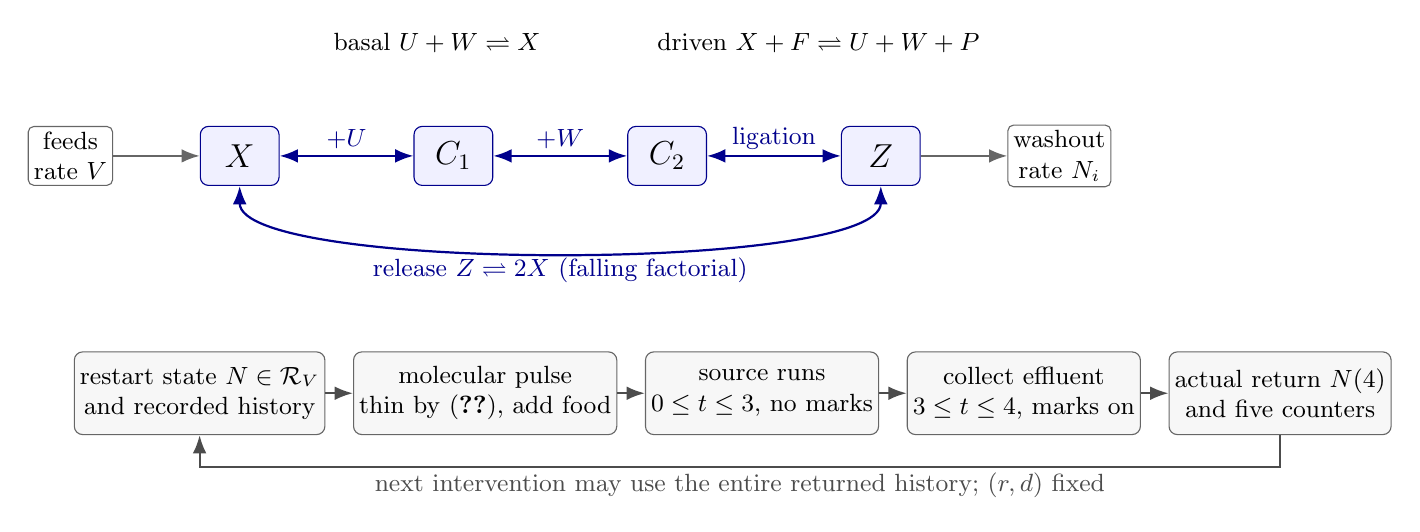
\begin{tikzpicture}[>=Latex,
  sp/.style={draw=blue!55!black,fill=blue!6,rounded corners=3pt,minimum width=1.0cm,minimum height=0.75cm,font=\large},
  st/.style={draw=black!60,fill=black!3,rounded corners=3pt,minimum width=2.45cm,minimum height=1.05cm,align=center,font=\small},
  lab/.style={font=\small},every node/.style={inner sep=2pt}]
\node[sp] (X) {$X$};
\node[sp,right=1.7cm of X] (C1) {$C_1$};
\node[sp,right=1.7cm of C1] (C2) {$C_2$};
\node[sp,right=1.7cm of C2] (Z) {$Z$};
\draw[<->,thick,blue!55!black] (X) -- node[lab,above] {$+U$} (C1);
\draw[<->,thick,blue!55!black] (C1) -- node[lab,above] {$+W$} (C2);
\draw[<->,thick,blue!55!black] (C2) -- node[lab,above] {ligation} (Z);
\draw[<->,thick,blue!55!black] (Z.south) .. controls ($(Z.south)+(0,-1.1)$) and ($(X.south)+(0,-1.1)$) .. node[lab,below,pos=0.5] {release $Z\rightleftharpoons 2X$ (falling factorial)} (X.south);
\node[lab,above=0.85cm of C1.north,anchor=south west,xshift=-1.6cm] {basal $U+W\rightleftharpoons X$};
\node[lab,above=0.85cm of C2.north,anchor=south west,xshift=-0.2cm] {driven $X+F\rightleftharpoons U+W+P$};
\node[draw=black!60,rounded corners=2pt,left=1.1cm of X,align=center,font=\small] (food) {feeds\\ rate $V$};
\draw[->,thick,black!60] (food) -- (X);
\node[draw=black!60,rounded corners=2pt,right=1.1cm of Z,align=center,font=\small] (out) {washout\\ rate $N_i$};
\draw[->,thick,black!60] (Z) -- (out);
\node[st,below=2.1cm of X.south west,anchor=north west,xshift=-1.6cm] (s1) {restart state $N\in\cR_V$\\ and recorded history};
\node[st,right=0.35cm of s1] (s2) {molecular pulse\\ thin by~\eqref{eq:pulse}, add food};
\node[st,right=0.35cm of s2] (s3) {source runs\\ $0\le t\le3$, no marks};
\node[st,right=0.35cm of s3] (s4) {collect effluent\\ $3\le t\le4$, marks on};
\node[st,right=0.35cm of s4] (s5) {actual return $N(4)$\\ and five counters};
\foreach \a/\b in {s1/s2,s2/s3,s3/s4,s4/s5}{\draw[->,thick,black!70] (\a) -- (\b);}
\draw[->,thick,black!70] (s5.south) -- ++(0,-0.4) -| node[lab,below,pos=0.25] {next intervention may use the entire returned history; $(r,d)$ fixed} (s1.south);
\end{tikzpicture}}
\caption{Reaction pathways and one physical cycle. All chemical links are reversible; the four-step templated path from $X+U+W$ to $2X$ is the autocatalytic completion. Food feeds and unit-rate washouts act continuously. Collection marks are switched on at time $3$; the actual endpoint starts the next cycle.}
\label{fig:protocol}
\end{figure}

\subsection{The history process and admitted controllers}\label{sec:history}
\begin{definition}[Returned-history process]\label{def:process}
Fix $V$, $(r,d)$, an initial state $N_0\in\cR_V$ and a controller $\pi$, an arbitrary function from finite lists of cycle records to admissible interventions. The returned-history process is the Markov chain on finite lists of records whose one-step kernel, from a list $h$ with current counts $N(h)$ (the counts of the newest record, or $N_0$ for the empty list), applies the intervention $\pi(h)$, samples the pulse and the four-unit marked source cycle from $N(h)$, and prepends the resulting record to $h$. Its $m$-step law from the empty list is the full normalized history law $\Prob$ over $m$ cycles.
\end{definition}
Every pulse and source outcome is retained, and every cycle starts from the actual returned counts. The controller sees the complete list of returned populations and counter values; no measurability or continuity is required of it. Section~\ref{sec:repeat} also treats a general measurable history space carrying possibly continuous observations, for which the requirement is that the next record, conditional on the current history and the chosen intervention, have exactly the literal pulse-and-source law, and that the current population equal the newest observed return. That requirement is a specification of the admissible physical model, not an assumption on success probabilities. No within-cycle control of rates is admitted.

\section{Main results}\label{sec:main}

For cycle $k\ge1$ let $S_k$ be the event that its record is successful in the sense of Definition~\ref{def:success}, and let $E_m=\bigcap_{k=1}^mS_k$. Under $\Prob$, a finite sequence of labelled reaction events and pulse category outcomes realizing the recorded history exists almost surely; we call such a sequence a physical trace. Let $\Pnet$ denote the signed net internal template synthesis along a trace: the sum over chemical events of the change of $\Iv$ they cause (pair 0 contributes $+1$ forward and $-1$ backward, pair 3 likewise, pair 5 contributes $-1$ forward and $+1$ backward, and pairs 1, 2, 4 contribute zero). Let $e(V)$ be the explicit finite sum of exponential and polynomial-exponential terms defined in Appendix~\ref{app:error}.

\begin{theorem}[Repeated finite-copy operation]\label{thm:main}
Fix $(r,d)$ in~\eqref{eq:parameters}, an integer $V\ge V_0:=200\,000\,000\,000$, a restart state $N_0\in\cR_V$ and a controller $\pi$. Then:
\begin{enumerate}[label=(\alph*)]
\item\label{it:one} (One cycle) For every $V\ge10^6$, every $N\in\cR_V$ and every admissible $p$, the probability that the cycle started from $N$ with intervention $p$ is successful is at least $1-e(V)$, where $0\le e(V)$ and $e(V)\le101e^{-V/10^{10}}$ for $V\ge V_0$.
\item\label{it:product} (Repetition) For every $m\in\N$,
\begin{equation}\label{eq:probability}
\Prob(E_m)\ge\bigl(1-e(V)\bigr)^m\ge1-m\,e(V).
\end{equation}
\item\label{it:totals} (Accounting) On $E_m$ every inequality of~\eqref{eq:success} holds in every cycle, hence the mission totals satisfy $\sum_kQ_{I,k}\ge m\lceil V/56\rceil$, $\sum_kQ_{X,k}\ge m\lceil V/1080\rceil$, $\sum_kC_{U,k},\sum_kC_{W,k}\le5mV$ and $\sum_kG_k\le m\lfloor V/5\rfloor$.
\item\label{it:synthesis} (Net synthesis) On $E_m$ a physical trace exists, and every physical trace of the recorded history satisfies
\begin{equation}\label{eq:sharp}
\Pnet\ \ge\ m\Bigl\lceil\frac V{56}\Bigr\rceil+\Bigl\lceil\frac V{28}\Bigr\rceil-\Iv_{N_0}
\ \ge\ m\Bigl\lceil\frac V{56}\Bigr\rceil+\Bigl\lceil\frac V{28}\Bigr\rceil-\Bigl\lfloor\frac{161V}{160}\Bigr\rfloor
\ \ge\ \Bigl(\frac{m+2}{56}-\frac{161}{160}\Bigr)V.
\end{equation}
In particular $\Pnet>0$ for every $m\ge55$ and every $N_0\in\cR_V$, and $\Pnet\ge13V/1750$ already for $m=2$ when $\Iv_{N_0}=8V/125$.
\end{enumerate}
\end{theorem}

\begin{corollary}[Logarithmic sizing and fixed-scale missions]\label{cor:scale}
For $m\ge1$ and $0<\delta<1$ put
\begin{equation}\label{eq:vlog}
V_{\log}(m,\delta)=\max\Bigl(V_0,\ \Bigl\lceil10^{10}\log\frac{101m}{\delta}\Bigr\rceil\Bigr).
\end{equation}
At every integer scale $V\ge V_{\log}(m,\delta)$, $\Prob(E_m)\ge1-\delta$. More generally, at any $V\ge V_0$ every mission length $m\le\lfloor(\delta/101)e^{V/10^{10}}\rfloor$ has $\Prob(E_m)\ge1-\delta$. At $V=V_0$,
\[
\Prob(E_{48000})\ge0.99,\qquad \Prob(E_{100})\ge0.999979.
\]
\end{corollary}

\begin{corollary}[Same-event operating ratios]\label{cor:ratios}
For $m\ge1$, on $E_m$ the mission totals $Q_I,Q_X,C_U,C_W,G$ are positive where they appear as denominators and satisfy
\begin{gather*}
\frac{Q_I}{4mV}\ge\frac1{224},\qquad \frac{Q_X}{4mV}\ge\frac1{4320},\qquad \frac{C_U}{Q_I},\ \frac{C_W}{Q_I}\le280,\qquad \frac{C_U+C_W}{Q_I}\le560,\\
\frac G{Q_I}\le\frac{56}5,\qquad \frac{C_U+C_W}{Q_X}\le10800,\qquad \frac G{Q_X}\le216.
\end{gather*}
For output demands $D_I$ template equivalents and $D_X$ free molecules at tolerance $\delta$, the integer scale $\max\bigl(V_{\log}(m,\delta),\,56D_I/m,\,1080D_X/m\bigr)$ is sufficient.
\end{corollary}

\begin{proposition}[Certificate bottleneck]\label{prop:bottleneck}
For every $V\ge0$, $e(V)\ge100e^{-V/10^{10}}$. Consequently, if $m\,e(V)\le\delta$ then $V\ge10^{10}\log(100m/\delta)$. This is a lower limit for the present certificate, not for a physical reactor.
\end{proposition}

\begin{remark}[Quantifiers]\label{rem:quantifiers}
The parameter pair is fixed once and arbitrary in its rectangle; the stochastic estimates in fact hold for $0\le d\le1/25$, and the lower bound $d\ge1/50$ in~\eqref{eq:parameters} is inherited from the thermochemical rectangle of~\citep{thermo2026}. The intervention class is the full box~\eqref{eq:pulsebounds} at every cycle, and the controller is an arbitrary function of the complete returned history. Part~\ref{it:one} holds from $V\ge10^6$; the larger floor $V_0$ is where the single-exponential envelope and the quantitative corollaries become available. Nothing in the theorem is conditional on success: $\Prob$ is the full normalized law, and $E_m$ is an event in it whose probability is bounded below. The costs are allowances on $E_m$; spending on unsuccessful runs is not bounded by them.
\end{remark}

\begin{remark}[Two formulations of the history]\label{rem:history}
Part~\ref{it:product} is proved for the concrete list-history process of Definition~\ref{def:process}. The same product bound is proved for every measurable history model that satisfies the literal conditional-law and actual-return requirements of Section~\ref{sec:history} (Proposition~\ref{prop:product}); such a model may record continuous within-cycle observations. The theorem does not separately construct a controlled continuous-time filtration for arbitrary raw-path controllers; the conditional-law formulation states exactly which physical models are admitted.
\end{remark}

\begin{remark}[Earlier linear rule]\label{rem:linear}
A first compiled version of Corollary~\ref{cor:scale} used the sufficient scale $\max(V_0,\lceil5\cdot10^6m/\delta\rceil)$, obtained from the bound $V\,e(V)\le5\cdot10^6$ on $V\ge V_0$. The logarithmic rule~\eqref{eq:vlog} rests on the exact absorption of every polynomial-exponential term into the phase term (Lemma~\ref{lem:absorb}); at $m=10^6$ and $\delta=10^{-2}$ it replaces $5\times10^{14}$ by $2.31\times10^{11}$ (Table~\ref{tab:sizing}).
\end{remark}

\begin{remark}[Proof map]
Sections~\ref{sec:pulse}--\ref{sec:counters} prove part~\ref{it:one} on a stopped uniformized device: the pulse leaves the material coordinates in a prepared band and the stock at least $3V/250$ (Section~\ref{sec:pulse}); the stock enters $Y\ge3V/50$ by time $11/4$ and stays above $V/20$ through time $4$, while the material coordinates return to their restart bands (Section~\ref{sec:recovery}); the five counters meet their thresholds (Section~\ref{sec:counters}). Section~\ref{sec:transfer} shows that the strict version of the stopped event transfers to the physical chronological process and that the analytical time split is exactly the physical four-unit law. Section~\ref{sec:repeat} conditions on actual returns for part~\ref{it:product}, telescopes the inventory for part~\ref{it:synthesis}, and proves the corollaries.
\end{remark}

\section{Pulse and material control}\label{sec:pulse}

\subsection{The retained stock}
\begin{lemma}[One-molecule retention factor]\label{lem:factor}
Let $0\le p\le1$, $0\le w\le9/5$ and $0\le s\le1/10$. Then
\[
1-p+p\,e^{-sw}\le\exp\Bigl\{-\Bigl(s-\frac{27}{25}s^2\Bigr)pw\Bigr\}.
\]
\end{lemma}
\begin{proof}
For $|z|\le9/50$ one has $e^{z}\le1+z+\tfrac35z^2$ (Appendix~\ref{app:tests}). With $z=-sw$, $|z|\le\tfrac9{50}$, so $1-p+pe^{-sw}\le1-psw+\tfrac35ps^2w^2\le1-psw+\tfrac35ps^2\cdot\tfrac95w=1-(s-\tfrac{27}{25}s^2)pw$, using $w^2\le\tfrac95w$. Finally $1+x\le e^x$.
\end{proof}

\begin{lemma}[Pulse stock tail]\label{lem:pulsestock}
Let $N\in\cR_V$ and let $p$ be admissible. The retained weighted stock $Y'$ after the pulse satisfies
\[
\Prob\bigl(Y'\le3V/250\bigr)\le e^{-1177V/10^{9}}.
\]
\end{lemma}
\begin{proof}
$Y'=\sum_aw_aB_a$ over molecules $a$, with $B_a$ independent Bernoulli retention indicators of parameters $p_a=q\ell_{i(a)}\in[49/200,1]$ and weights $w_a\in\{1,9/8,7/5,9/5\}$ for catalytic molecules and $0$ otherwise. The exact moment generating function is $\E e^{-sY'}=\prod_a(1-p_a+p_ae^{-sw_a})$; Lemma~\ref{lem:factor} bounds it by $\exp\{-(s-\tfrac{27}{25}s^2)\sum_ap_aw_a\}$, and $\sum_ap_aw_a\ge\tfrac14\cdot\tfrac{49}{50}\cdot Y_N\ge\tfrac{49}{4000}V$ because $Y_N\ge V/20$ on $\cR_V$. The exponential Markov inequality at $s=1/100$ and level $a=3V/250$ gives the exponent $sa-(s-\tfrac{27}{25}s^2)\tfrac{49V}{4000}=-\tfrac{1177}{10^9}V$.
\end{proof}
The exponent uses the actual retained mean rather than the sum of squared weights; the retained stock $3V/250$ is one quarter of the deterministic prepared stock $49/4000$, leaving room for the fluctuations of about $V^{1/2}$ molecules.

\subsection{The retained material}
\begin{lemma}[Pulse material tails]\label{lem:pulsematerial}
Let $N\in\cR_V$, $V\ge10^6$, and let $p$ be admissible. After the pulse, each of $A,B$ lies in the prepared band $[24V/25,\,51V/50]$ except with probability at most $4e^{-V/100000}$ in total.
\end{lemma}
\begin{proof}
Each material coordinate after the pulse is $\sum_aw_aB_a+D$, with material weights $w_a\in\{1,2\}$ and an integer dose $D=\lfloor V(1-q+e)\rfloor$. Its mean is $q\sum_a\ell_{i(a)}w_a+D$; over the restart band, the box~\eqref{eq:pulsebounds} and the floor, the mean lies in $[\tfrac{31213}{32000}V-1,\ \tfrac{3231}{3200}V]$, whose distance from each end of the prepared band exceeds $V/100-1$. A deviation of magnitude $V/100-1$ for a sum of independent bounded terms with weights at most $2$ costs at most $e^{-V/100000}$ per sign by the bounded-difference exponential inequality~\citep{hoeffding1963}; two coordinates and two signs give $4e^{-V/100000}$.
\end{proof}
Neither lemma conditions on a good pulse: bad pulses keep their mass and are counted in $e(V)$.

\subsection{The corridor, uniformization and material exit}\label{sec:corridor}
Stop the process temporarily when either $A$ or $B$ leaves the corridor $[9V/10,\,11V/10]$. On the corridor every count is at most $11V/10$ and the sum of all propensities is at most $3000V$ (the actual sum is below $175V$; the slack is irrelevant). This permits uniformization~\citep{jensen1953,grassmann1977}: a Poisson clock of rate $q_c=3000V$ selects channel $j$ with probability $a_j(N)/q_c$ and otherwise makes a null step, giving a finite stopped kernel $P=I+\Lgen/q_c$ whose expectations at time $t$ are Poisson mixtures of kernel powers. Counters remain attached to the selected labels. For a linear observable $H$ and tilt $s$, the exponential test satisfies
\begin{equation}\label{eq:exptest}
\frac{\Lgen e^{sH}(N)}{e^{sH(N)}}=\sum_ja_j(N)\bigl(e^{s\Delta_jH}-1\bigr)
\le s\,\Lgen H(N)+\frac35s^2\sum_ja_j(N)(\Delta_jH)^2\qquad(|s\Delta_jH|\le9/50),
\end{equation}
by the quadratic exponential inequality. One kernel step multiplies a test by at most $1+\Lgen e^{sH}/(q_ce^{sH})$; iteration, the exponential Markov inequality and Poisson summation give tails. Indicators of activity kill a test on exit, and every exit probability appears explicitly in the budget.

\begin{lemma}[Material corridor exit]\label{lem:corridor}
From the prepared band, the probability that $A$ or $B$ leaves the corridor during a run of four time units is at most
\begin{equation}\label{eq:M}
M(V)=4e^{-V/2000}+48000V\,e^{-V/2000+1/50}.
\end{equation}
\end{lemma}
\begin{proof}
For $H\in\{A,B\}$ use the barriers $U_H=e^{(H-11V/10)/100}$ and $L_H=e^{-(H-9V/10)/100}$. At a prepared start each is at most $e^{-V/2000}$; at an exit their sum is at least one. Outside the inner band $|H-V|\le V/20$ the restoring drift $\Lgen H=V-H$ dominates the quadratic remainder in~\eqref{eq:exptest}, so the tilted drift is nonpositive; inside it each barrier is at most $e^{-V/2000}$ and a material jump of size at most $2$ changes its exponent by at most $1/50$, so the generator of each barrier is at most $q_ce^{-V/2000+1/50}$. Integrating over four time units gives $4\cdot3000V\cdot4\,e^{-V/2000+1/50}$ for the four barriers and $4e^{-V/2000}$ for the starts.
\end{proof}

\begin{lemma}[Terminal material return]\label{lem:terminal}
On the corridor, from a start with $|H_0-V|\le V/25$, the probability that $|H(4)-V|\ge V/160$ for $H=A$ or $H=B$, on the event of no corridor exit, is at most $4(e^{-V/320000}+e^{-V})$.
\end{lemma}
\begin{proof}
Let $T_s=\one_{\rm corridor}e^{s(H-V)}$. The drift $V-H$ contracts the tilt: the compensated test $e^{-2s^2V}T_s$ satisfies $P^nT_s\le e^{2s^2V}T_{(1-1/q_c)^ns}$ for $|s|\le1/100$. After $n\ge11700V$ steps the contraction factor is at most $e^{-3.9}\le1/40$. With $s=\pm1/1000$ the exponent for the terminal threshold $|H-V|\ge V/160$ is at most $-V/160000+2V/10^6+V/10^6\le-V/320000$. The Poisson clock of mean $12000V$ produces fewer than $11700V$ steps with probability at most $e^{-V}$. Two coordinates and two signs give the factor $4$.
\end{proof}
Both the prepared band and the narrow terminal band are kept; the exact cancellation $\Lgen A=V-A$ alone would not imply concentration at the return time.

\section{Recovery, residence and phase transport}\label{sec:recovery}

\subsection{Guarded growth and the stock exponential test}
\begin{lemma}[Guarded growth of the count stock]\label{lem:growth}
On the corridor, if $Y_N\le3V/50$ then $\Lgen Y_N\ge\tfrac23Y_N$. Moreover, on the corridor with small stock the basal creation channel contributes at least $V/10^9$ to $\Lgen Y_N$, and the rate-weighted squared jumps of $Y$ are at most $6Y_N+V/10^8$.
\end{lemma}
\begin{proof}
By~\eqref{eq:drift}, $\Lgen Y_N=V\,Y(f_{r,d}(c))+rN_X/(5V)$ with $c=N/V$, and the last term is nonnegative. The companion paper~\citep[Lemma~4.6]{recovery2026} proves $Y(f_{r,d}(c))\ge\tfrac23Y(c)$ on the concentration corridor whenever $Y(c)\le3/50$, by exhibiting a nonnegative parameterized surplus; the mechanism is that low stock forces both free foods above $3/4$ (the exact floors are $119/150$ and $57/70$), so the templated path carries positive net weighted flux. The basal channel then has propensity $\eps N_UN_W/V\ge\eps(3/4)^2V>V/10^9$ with $Y$-increment $1$. Every $Y$-jump has magnitude at most $9/5$; summing squared increments against propensities on the corridor gives the stated linear bound.
\end{proof}
This is a generator inequality, not a claim that random paths grow monotonically.

\begin{lemma}[Stock exponential test]\label{lem:stocktest}
On the corridor, for $0\le s\le1/100$ and $Y_N\le3V/50$,
\[
\Lgen e^{-sY_N}\le-\tfrac58\,s\,Y_N\,e^{-sY_N}.
\]
\end{lemma}
\begin{proof}
Apply~\eqref{eq:exptest} to $H=-Y$: the right side is $-s\Lgen Y_N+\tfrac35s^2(6Y_N+V/10^8)$. By Lemma~\ref{lem:growth}, $-s\Lgen Y_N\le-\tfrac23sY_N-sV/10^9$. At $s\le1/100$ the coefficient of $Y_N$ is at most $-(\tfrac23-\tfrac35\cdot6\cdot\tfrac1{100})s=-\tfrac{473}{750}s\le-\tfrac58s$, and $\tfrac35s^2V/10^8\le sV/10^9$, so the basal term pays for the additive noise source.
\end{proof}

\subsection{Seeded recovery}
\begin{proposition}[Seeded recovery deadline]\label{prop:entry}
From a prepared start on the corridor with $Y\ge3V/250$, the probability that the stopped process is still active and below $Y=3V/50$ at time $11/4$ is at most
\[
e^{-3V/5\,000\,000}+e^{-V/2}.
\]
\end{proposition}
\begin{proof}
Let $T_s=\one_{\{\text{active},\,Y<3V/50\}}e^{-sY}$. Lemma~\ref{lem:stocktest} and uniformization give $PT_s\le T_t$ whenever $t\le(1+\tfrac{5/8}{q_c})s$, for $s\le1/100$. Start at the deadline with tilt $1/1000$ and transport it backward through $8100V$ steps, increasing the tilt by the factor $1+\tfrac{5/8}{3000V}$ per step and capping it at $101/20000$. Grouping the steps into $27$ blocks of $300V$ and applying Bernoulli's inequality blockwise, $(1+\tfrac{5}{24000V})^{300V}\ge\tfrac{17}{16}$, and $(17/16)^{27}>101/20$, so the cap is reached before the start. Hence $P^{8100V}T_{1/1000}\le T_{101/20000}$ at the start, and by the exponential Markov inequality the probability of being active below $3V/50$ after $8100V$ steps is at most
\[
\exp\Bigl\{\frac1{1000}\cdot\frac{3V}{50}-\frac{101}{20000}\cdot\frac{3V}{250}\Bigr\}=e^{-3V/5\,000\,000}.
\]
The Poisson clock of mean $8250V=\tfrac{11}4\cdot3000V$ produces fewer than $8100V$ steps with probability at most $e^{-V/2}$.
\end{proof}
The certified exponent is small because the tilt is small; the mechanism is nevertheless comfortable, since the drift coefficient $5/8$ over the deadline $11/4$ gives a growth factor above $5.13$ where the ratio of target to prepared stock is $5$. The random entry state is continued as it is; no replacement start at the target is used.

\begin{lemma}[Residence]\label{lem:residence}
From an active state with $Y\ge3V/50$, the probability that the stopped process is still active and has $Y\le V/20$ at some fixed later time $t\le4$ is at most $e^{-V/10000}+12000V\,e^{-V/10000+9/500}$.
\end{lemma}
\begin{proof}
Use $H_Y=\max(e^{-Y/100},e^{-3V/5000})$. Below the cap Lemma~\ref{lem:stocktest} applies and the drift is nonpositive; above it a jump changes $Y$ by at most $9/5$, so $\Lgen H_Y\le q_ce^{-3V/5000+9/500}$. At the start $H_Y=e^{-3V/5000}$; at a state with $Y\le V/20$, $H_Y\ge e^{-V/2000}$. Integration over time at most $4$ and division by $e^{-V/2000}$ give the bound, since $-3/5000+1/2000=-1/10000$.
\end{proof}
Applying Proposition~\ref{prop:entry} to the actual state at time $11/4$ and Lemma~\ref{lem:residence} through the remaining $5/4$ units yields the recovery-and-residence budget $R(V)$ of Appendix~\ref{app:error}; material exits are paid separately by Lemma~\ref{lem:corridor}. The times $11/4$ and $1/4$ partition the analysis only (Section~\ref{sec:transfer}).

\subsection{Positive phase transport to free template}\label{sec:phase}
Large $Y$ does not imply large $N_X$ at the same instant: the stock may sit in the bound phases $C_1,C_2,Z$. A constant linear corrector fails here (its boundary penalty exceeds the available stock integral), and the successful replacement is a short-window transport estimate that keeps every phase endpoint.

\begin{lemma}[Phase comparison drifts]\label{lem:phase}
On the corridor,
\begin{equation}\label{eq:phase-drift}
\begin{aligned}
\Lgen N_X&\ge-70N_X+20N_{C_1}+38N_Z,&
\Lgen N_{C_1}&\ge-70N_{C_1}+20N_{C_2},\\
\Lgen N_{C_2}&\ge-70N_{C_2},&
\Lgen N_Z&\ge-70N_Z+20N_{C_2}.
\end{aligned}
\end{equation}
\end{lemma}
\begin{proof}
Read off~\eqref{eq:generator} with Table~\ref{tab:rates}. For $N_X$ the negative terms are $-(\eps/10)N_X-20N_XN_U/V-2rN_X(N_X-1)/V-dN_X-N_X$; with $N_U,N_X\le11V/10$, $r\le21$ and $d\le1/25$ their coefficient is at most $69.25$, and the positive terms include $20N_{C_1}$ and $2rN_Z\ge38N_Z$. The other three follow in the same way with coefficients $43$, $41$ and $24$; the common value $70$ is used for all.
\end{proof}

\begin{lemma}[Backward weights]\label{lem:weights}
Put $q_c=3000V$, $a=1-70/q_c$, and define the weight vector $w(n)=(w_X,w_{C_1},w_{C_2},w_Z)(n)$ by $w(0)=(1,0,0,0)$ and
\[
w(n+1)=\Bigl(aw_X,\ aw_{C_1}+\tfrac{20}{q_c}w_X,\ aw_{C_2}+\tfrac{20}{q_c}(w_{C_1}+w_Z),\ aw_Z+\tfrac{38}{q_c}w_X\Bigr).
\]
Then $w(n)$ is nonnegative with $w_X+w_{C_1}+w_{C_2}+w_Z\le1$, and
\begin{equation}\label{eq:weights}
w(n)=a^n\Bigl(1,\ \frac{20n}{q_ca},\ \frac{580n(n-1)}{q_c^2a^2},\ \frac{38n}{q_ca}\Bigr).
\end{equation}
For $89V\le n\le91V$, every coordinate of $w(n)$ is at least $1/35$ times the corresponding weight of $Y$, so $w(n)\cdot N\ge Y_N/35$.
\end{lemma}
\begin{proof}
The closed form satisfies the recursion, and $q_c$ times the loss of mass in one step is $12w_X+50w_{C_1}+70w_{C_2}+50w_Z\ge0$. For $n\le91V$, $a^n\ge e^{-11/5}\ge1/12$ by $\log a\ge1-1/a$ and $e^{11/5}\le12$. With $n\ge89V$ and $n-1\ge88V$, the four coordinates are at least $\tfrac1{12}$, $\tfrac1{12}\cdot\tfrac{20\cdot89}{3000}$, $\tfrac1{12}\cdot\tfrac{580\cdot89\cdot88}{9\cdot10^6}$ and $\tfrac1{12}\cdot\tfrac{38\cdot89}{3000}$, which exceed $\tfrac1{35}(1,\tfrac98,\tfrac75,\tfrac95)$ coordinatewise; the tightest is $C_2$, with $0.0421$ against $0.0400$.
\end{proof}
The weights are the adjoint iteration of the one-step comparison kernel of~\eqref{eq:phase-drift}: $w(n)\cdot N$ is a lower bound for the expected free count $n$ steps ahead, and Figure~\ref{fig:weights} shows how each phase contributes. Any catalytic phase can fund a future free-template observation; the estimate does not assume that stock is initially free.

\begin{figure}[tb]
\centering
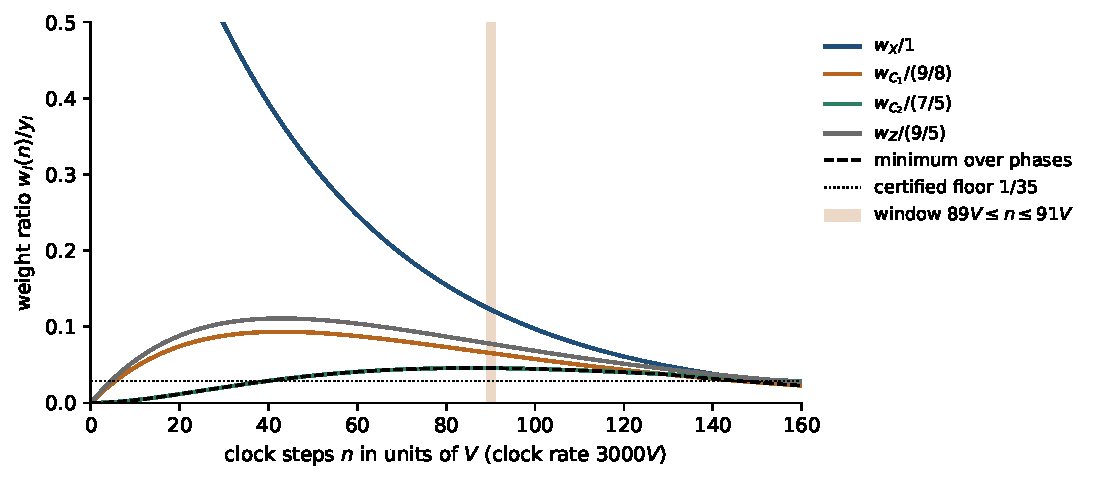
\includegraphics[width=\linewidth]{phase_weights.pdf}
\caption{Backward phase-transport weights~\eqref{eq:weights} in the large-$V$ form $n=\tau V$, divided by the stock weights $(1,9/8,7/5,9/5)$. Free template contributes immediately and decays; the bound phases contribute after a lag through the actual release path. In the certified window $89V\le n\le91V$ every ratio exceeds $1/35$, so $w(n)\cdot N\ge Y_N/35$.}
\label{fig:weights}
\end{figure}

\begin{proposition}[Low free template after a phase window]\label{prop:lowfree}
Let $N$ be an active corridor state with $Y_N\ge V/20$. For $89V\le n\le91V$, the probability that the stopped process is still active after $n$ clock steps with $N_X\le V/1000$ is at most $e^{-V/10^{10}}$.
\end{proposition}
\begin{proof}
Apply~\eqref{eq:generator} to $e^{-s\,w\cdot N}$ for a nonnegative weight vector $w$ of mass at most one. Every jump changes $w\cdot N$ by at most $2$, and the total rate is at most $q_c$, so for $0\le s\le1/100$
\begin{equation}\label{eq:phase-mgf}
\Lgen e^{-sw\cdot N}\le e^{-sw\cdot N}\bigl\{-s\,D_w(N)+7200Vs^2\bigr\},
\end{equation}
where $D_w$ is the weighted right side of~\eqref{eq:phase-drift}. One kernel step applied to $e^{-s\,w(k)\cdot N}$ is bounded by $e^{-s\,w(k+1)\cdot N}\bigl(1+\tfrac{7200V}{q_c}s^2\bigr)=e^{-s\,w(k+1)\cdot N}\bigl(1+\tfrac{12}5s^2\bigr)$, because $w(k+1)-w(k)$ is exactly $1/q_c$ times the adjoint of the comparison drift~\eqref{eq:phase-drift} applied to $w(k)$, so the drift term of~\eqref{eq:phase-mgf} is absorbed by the change of weights. After $n$ steps, $\E[\one_{\rm active}e^{-sN_X(n)}]\le e^{-sw(n)\cdot N}(1+\tfrac{12}5s^2)^n$. With $s=10^{-6}$, $w(n)\cdot N\ge V/700$ and the threshold $N_X\le V/1000$, the exponential Markov inequality gives the exponent
\[
\Bigl(10^{-9}-\frac1{7\cdot10^{8}}+\frac{12}5\cdot91\cdot10^{-12}\Bigr)V\le-\frac V{10^{10}}.\qedhere
\]
\end{proof}

\begin{proposition}[Occupation and free collection]\label{prop:free}
From an active state with $Y\ge V/20$ at time $3$ that remains active through time $4$, the free-template counter fails its threshold, $Q_X<\lceil V/1080\rceil$, with probability at most
\begin{equation}\label{eq:F}
F(V)=e^{-V/(4\cdot10^{7})}+100e^{-V/10^{10}}+e^{-V}+e^{-V/200}.
\end{equation}
\end{proposition}
\begin{proof}
Condition, at every clock step of the collection unit after a burn-in of $90V$ steps, on the state $90V$ steps earlier; Proposition~\ref{prop:lowfree} bounds the conditional probability of a low-free state by $e^{-V/10^{10}}$ whenever the earlier state had $Y\ge V/20$, which residence guarantees. If $B$ counts low-free steps among the $n$ collection steps, then $\E B\le ne^{-V/10^{10}}$ and Markov's inequality gives $\Prob(B\ge n/100)\le100e^{-V/10^{10}}$, with no independence between the steps. On the complementary event at least $99\%$ of the collection steps have $N_X>V/1000$, so the free-washout mark has mean at least $1/3000$ per such step. A marked lower-tail tilt of size $1/1000$ applied to the statistic $Q_X+B/(3\cdot10^6)$ gives, for $n\ge2990V$ collection steps, the shortfall bound $\exp\{\tfrac1{1000}(\lceil V/1080\rceil+\tfrac{n/100}{3\cdot10^6})-\tfrac{33n}{10^{11}}\}\le e^{-V/(4\cdot10^7)}$ for $V\ge10^6$. The precollection quarter unit and the collection unit have clock means $750V$ and $3000V$; their lower tails contribute $e^{-V}$ and $e^{-V/200}$.
\end{proof}
The statistic $Q_X+B/(3\cdot10^6)$ is a proof device; the counted output is the actual free washout. The term $100e^{-V/10^{10}}$ is the dominant term of $e(V)$ (Proposition~\ref{prop:bottleneck}); the burn-in of $90V$ steps is a lag of about $0.03$ time units and is why collection is preceded by three units of uncollected recovery rather than $11/4$.

\section{Marked outputs, supplies and the joint counter budget}\label{sec:counters}

\begin{lemma}[Template output]\label{lem:template}
During residence above $Y=V/20$ the template washout intensity satisfies $\Iv_N\ge V/28$, and the template counter fails its threshold, $Q_I<\lceil V/56\rceil$, on the active path with probability at most $e^{-V/100000}$ for $V\ge10^6$.
\end{lemma}
\begin{proof}
Comparing weights, $Y_N\le\tfrac75\Iv_N$, so $\Iv_N\ge V/28$. The washout of $X,C_1,C_2,Z$ has total propensity $\Iv_N$ in molecules and mean template mark at least $\Iv_N$ per unit time, hence mean mark at least $1/84000$ per clock step. A lower-tail tilt of size $1/1000$ on a nonnegative mark bounded by $2$ multiplies the test by at most $e^{-33/(2.8\cdot10^{9})}$ per active step. Poisson summation over the collection clock of mean $3000V$ gives the exponent $\tfrac{V/56+1}{1000}+3000V(e^{-33/(2.8\cdot10^9)}-1)\le-V/100000$, where the $+1$ certifies the integer ceiling.
\end{proof}

\begin{lemma}[Food and gross service]\label{lem:supply}
Over the whole cycle, each food counter exceeds $5V$ with probability at most $e^{-V/300}$, and the gross driven-service counter exceeds $\lfloor V/5\rfloor$ with probability at most $e^{-V/2000}$, for $V\ge10^6$.
\end{lemma}
\begin{proof}
For a counter with intensity at most $cV$, initial value $z$ and threshold $K$, an upper-tail tilt of size $s$ over four time units has exponent $-sK+4cV(e^s-1)+sz$. Each feed has constant rate $V$ and the pulse dose is at most $151V/200$; with $c=1$, $s=1/50$, $K=5V$ the exponent is at most $-V/300$. On the corridor the gross pair-5 intensity is $dN_X+d\eta N_UN_W/V\le\tfrac1{25}(\tfrac{11}{10}+\tfrac{121}{100}\eta)V<\tfrac9{200}V$; with $c=9/200$, $s=1/20$, $z=0$ and $K=V/5-1$ the exponent is at most $-V/2000$, the $-1$ certifying the integer floor.
\end{proof}

\begin{proposition}[Joint counter budget on one law]\label{prop:counters}
On the stopped device, from a prepared start, the probability that the path is active through time $4$ and at least one of the five counters fails its threshold in~\eqref{eq:success} is at most
\begin{equation}\label{eq:J}
J(V)=F(V)+e^{-V/100000}+2e^{-V/300}+e^{-V/2000}.
\end{equation}
\end{proposition}
\begin{proof}
All five counters are functions of the same sequence of labelled events, retained through the three analytical segments $[0,11/4]$, $[11/4,3]$, $[3,4]$ with the actual intermediate chemical states. The output marginals hold their counters at zero until collection and the supply marginals accumulate from the pulse dose. Propositions~\ref{prop:free} and Lemmas~\ref{lem:template}--\ref{lem:supply} bound each failure on that joint law; their sum is a union bound within it, not a product of marginal laws.
\end{proof}

\begin{proposition}[Prepared cycle]\label{prop:prepared}
From a start on the prepared band with $Y\ge3V/250$, the probability that the stopped path exits, fails to return to $\cR_V$ at time $4$ while active, or fails a counter, is at most $J(V)+T(V)$, where
\begin{equation}\label{eq:T}
T(V)=M(V)+R(V)+4\bigl(e^{-V/320000}+e^{-V}\bigr)
\end{equation}
is the restart budget, with $R(V)$ the recovery-and-residence budget of Appendix~\ref{app:error}.
\end{proposition}
\begin{proof}
Lemma~\ref{lem:corridor} pays material exits, Proposition~\ref{prop:entry} and Lemma~\ref{lem:residence} pay stock failures through the actual entry and deadline states, Lemma~\ref{lem:terminal} pays the terminal material bands, and Proposition~\ref{prop:counters} pays the counters. The events are combined by a union bound on the joint three-segment law.
\end{proof}

\begin{proposition}[Stopped one-cycle bound]\label{prop:stopped}
For $V\ge10^6$, $N\in\cR_V$ and admissible $p$, integrating over the pulse law, the stopped device fails the strict event (active terminal state, $N(4)\in\cR_V$, all counter thresholds) with probability at most
\begin{equation}\label{eq:e}
e(V)=e^{-1177V/10^{9}}+4e^{-V/100000}+J(V)+T(V).
\end{equation}
\end{proposition}
\begin{proof}
Bad pulses (Lemmas~\ref{lem:pulsestock} and~\ref{lem:pulsematerial}) are charged one; good pulses start on the prepared band with $Y\ge3V/250$ and are charged $J(V)+T(V)$ by Proposition~\ref{prop:prepared}. Summing against the pulse masses, which total one, gives~\eqref{eq:e}.
\end{proof}

\section{From the stopped device to the physical law}\label{sec:transfer}

\subsection{The strict event}
\begin{remark}[The closed restart event does not transfer]\label{rem:boundary}
The restart stock inequality is closed ($Y\ge V/20$) and the residence stop is at $Y\le V/20$, so a stopped path can end in $\cR_V$ while frozen at the boundary. A three-state exact model in the accompanying workspace has stopped closed-restart probability $1$ and unrestricted probability $1/2$ after two steps. This refutes the generic transfer of the closed event; it is not a counterexample to the reactor theorem. The strictly active event in that model has probability $1/4$ under both laws.
\end{remark}
\begin{lemma}[Strict terminal activity implies agreement]\label{lem:strict}
Inactive states are absorbing in the stopped kernel. Hence, on the event that the terminal state is active, no earlier exit occurred, and the stopped and literal updates, including every counter increment, agree at every step. The probability of losing the strict event is already contained in $T(V)$.
\end{lemma}

\subsection{Killed chronology and the stopped clock}
\begin{lemma}[Renewal identity]\label{lem:renewal}
Let $D$ be a set of states on which the total rate is bounded. The law of the chronological jump process killed at its first exit from $D$ and the law of the uniformized stopped clock, both with marks and waiting times, satisfy the same first-event renewal equation, whose solution on a bounded time interval is unique. Hence the two killed laws agree, and the stopped-clock expectation of any nonnegative terminal payoff vanishing off $D$ is at most the corresponding expectation under the unrestricted chronological process.
\end{lemma}
\begin{proof}
Expanding on the first waiting time and first label gives the equation directly for each construction; a null step of the clock carries no mark and no state change, and the survival kernel at the genuine rate solves the resolvent equation of the clock rate, including the case of equal rates. Uniqueness follows by iterating the residual, whose remainder after $k$ iterations on an interval of length $t$ is bounded by the tail of the exponential series of the rate bound. Domination by the unrestricted process is monotonicity of a payoff that vanishes off $D$.
\end{proof}
The identity preserves waiting times and labels, not merely a state marginal, which is what the counters require.

\subsection{Nonexplosion and the chronological semigroup}
\begin{lemma}[Nonexplosion]\label{lem:nonexplosion}
For every $V>0$, $r,d\ge0$ and every count start, the twenty-channel chronological process has almost surely finitely many events on every bounded time interval.
\end{lemma}
\begin{proof}
Only the two constant-rate feeds increase the total material $A_N+B_N$; their number on a bounded interval is Poisson and almost surely finite. Every region of bounded material height contains finitely many count states and has bounded total rate, so the process makes finitely many jumps before the next feed. No global rate bound is assumed~\citep[cf.][]{norris1997,anderson2015}.
\end{proof}

\begin{proposition}[Chronological semigroup and exhaustion]\label{prop:semigroup}
Exhaust the state space by regions of bounded material height. The killed endpoint laws increase with the region and their supremum is the unrestricted chronological law. The composition identity $P_{t+s}=P_tP_s$ holds for the bounded uniformized clock by Poisson convolution, passes to each killed law, and passes to the limit by monotone convergence, a common larger region handling the two factors. Consequently the analytical split $11/4+1/4$ of the uncollected run is exactly the physical three-unit law, the collection unit with marks switched on is the physical marked law, and erasing the counters at time $4$ recovers the original count endpoint.
\end{proposition}
Every step of Lemmas~\ref{lem:strict}--\ref{lem:nonexplosion} and Proposition~\ref{prop:semigroup} is compiled in Lean (Appendix~\ref{app:formal}); in the companion papers~\citep{finitecopy2026,exporter2026} the identification was a conventional argument.

\subsection{The literal cycle bound}
\begin{theorem}[One cycle on the physical law]\label{thm:onecycle}
For $V\ge10^6$, every $N\in\cR_V$ and every admissible $p$, the literal pulse-and-source cycle measure gives the successful records of Definition~\ref{def:success} probability at least $1-e(V)$.
\end{theorem}
\begin{proof}
By Proposition~\ref{prop:stopped} the strict stopped event has probability at least $1-e(V)$. By Lemma~\ref{lem:strict} and Lemma~\ref{lem:renewal} the strict event is dominated by the corresponding event of the killed chronological process, and by Proposition~\ref{prop:semigroup} the composed killed laws are the literal four-unit marked law. The strict event implies the successful-record event, and the pulse integration is the same on both sides.
\end{proof}
This is part~\ref{it:one} of Theorem~\ref{thm:main}.

\section{Repetition, inventory and quantitative consequences}\label{sec:repeat}

\subsection{Conditioning on actual returns}
\begin{proposition}[Product bound]\label{prop:product}
For the returned-history process of Definition~\ref{def:process}, and for every measurable history model with the literal conditional law and actual-return property, $\Prob(E_m)\ge(1-e(V))^m$ for all $m$.
\end{proposition}
\begin{proof}
Let $K(h,\cdot)$ be the one-step history kernel and $S$ the set of histories whose newest record is successful. A successful record places the actual next state in $\cR_V$, so Theorem~\ref{thm:onecycle} gives $K(h,S)\ge1-e(V)$ whenever the current state of $h$ is in $\cR_V$. Integrating over successful prefixes,
\[
\Prob(E_{m+1})=\int_{E_m}K(h,S)\,\Prob(\dd h)\ge(1-e(V))\Prob(E_m),
\]
and induction gives the product. The measure restricted to successful prefixes is an unnormalized submeasure of the full law whose mass is the success probability; it is never renormalized into a conditional sampling procedure, and no independence between cycles is used. Bernoulli's inequality $(1-e)^m\ge1-me$ gives the linear form.
\end{proof}
This is part~\ref{it:product}; part~\ref{it:totals} is summation of~\eqref{eq:success} over the records of a history in $E_m$.

\subsection{Pathwise inventory and net synthesis}
\begin{lemma}[Inventory identity]\label{lem:inventory}
Along any physical trace of a recorded history,
\begin{equation}\label{eq:inventory}
\Pnet=\Iv_{\rm final}-\Iv_{\rm initial}+Q_{\rm all\ washout}+\Iv_{\rm withdrawn}+\Iv_{\rm extra\ loss},
\end{equation}
where $Q_{\rm all\ washout}$ counts the template weight of every washout in every cycle, collected or not, and the last two terms count the template weight of withdrawn and extra-lost molecules at every pulse.
\end{lemma}
\begin{proof}
Each chemical event changes $\Iv$ by its synthesis mark, each feed by zero, each washout by minus its template weight, and each pulse by minus the template weight of the molecules that leave. Telescoping over all events and pulse boundaries gives~\eqref{eq:inventory}.
\end{proof}

\begin{proposition}[Net synthesis]\label{prop:synthesis}
On $E_m$, every physical trace satisfies~\eqref{eq:sharp}.
\end{proposition}
\begin{proof}
All removal terms in~\eqref{eq:inventory} are nonnegative and $Q_{\rm all\ washout}\ge\sum_kQ_{I,k}\ge m\lceil V/56\rceil$. The final state is in $\cR_V$, and comparing $(40,45,56,72)$ with $(56,56,56,112)$ gives $40Y_N\le56\Iv_N$, so $\Iv_{\rm final}\ge V/28$, hence $\ge\lceil V/28\rceil$ since inventory is an integer. Initially $\Iv_{N_0}\le A_{N_0}\le161V/160$, and the integer inventory is at most $\lfloor161V/160\rfloor$. Dropping the ceilings gives the real form. The formal event contains the existence of a trace, so the universal statement over traces is not vacuous.
\end{proof}
At $m=55$ the real bound equals $13V/1120>0$, and for $\Iv_{N_0}=8V/125$ two cycles give $2\lceil V/56\rceil+\lceil V/28\rceil-8V/125\ge13V/1750$. The statement is net synthesis inside the maintained source; it does not label exported molecules, isolate the contribution of the templated path, or prove pathway necessity.

\subsection{The single exponential and the sizing rule}
\begin{lemma}[Two-term envelope]\label{lem:envelope}
For every $V\ge0$,
\begin{equation}\label{eq:envelope}
e(V)\le100e^{-V/10^{10}}+10^6(V+1)e^{-V/(4\cdot10^{7})}.
\end{equation}
\end{lemma}
\begin{proof}
Every term of $e(V)$ other than $100e^{-V/10^{10}}$ decays at least as fast as $e^{-V/(4\cdot10^7)}$. The constant coefficients sum to $31$, and the two polynomial prefactors, with $e^{1/50},e^{9/500}\le2$, contribute at most $216000V$; both are below $10^6(V+1)$.
\end{proof}

\begin{lemma}[Residual absorption]\label{lem:absorb}
For $V\ge V_0$, $10^6(V+1)e^{-V/(4\cdot10^7)}\le e^{-V/10^{10}}$; hence $e(V)\le101e^{-V/10^{10}}$.
\end{lemma}
\begin{proof}
Put $x=249V/10^{10}$, so that $e^{-V/(4\cdot10^7)}=e^{-V/10^{10}}e^{-x}$ and $x\ge4980$. The Taylor term gives $e^x\ge x^6/720\ge4980^5x/720$, and $4980^5\cdot249V/(720\cdot10^{10})>10^8V\ge10^6(V+1)$. This is an exact polynomial comparison on the whole domain $V\ge V_0$.
\end{proof}

\begin{proof}[Proof of Corollary~\ref{cor:scale}]
By Lemma~\ref{lem:absorb} and~\eqref{eq:vlog}, $V/10^{10}\ge\log(101m/\delta)$ gives $m\,e(V)\le101me^{-V/10^{10}}\le\delta$; the mission-length form is the same inequality solved for $m$. For the fixed-scale statements one exact rational certificate suffices:
\begin{equation}\label{eq:taylor}
e^{20}\ge\sum_{k=0}^{36}\frac{20^k}{k!}>484\,800\,000,
\end{equation}
so $e(V_0)\le101e^{-20}\le1/4\,800\,000$. Multiplying by $48\,000$ gives $1/100$; multiplying by $100$ gives $1/48\,000<21/10^6$.
\end{proof}

\begin{proof}[Proof of Proposition~\ref{prop:bottleneck}]
The term $100e^{-V/10^{10}}$ is a summand of $F(V)$ and all other summands of $e(V)$ are nonnegative. If $me(V)\le\delta$ then $100me^{-V/10^{10}}\le\delta$, which is the stated inequality.
\end{proof}

\begin{table}[tb]
\centering\small
\begin{tabular}{rrr}
\toprule
Cycles $m$ & Earlier linear rule $\max(V_0,\lceil5\cdot10^6m/\delta\rceil)$ & Logarithmic rule, sufficient scale\\
\midrule
100 & 200,000,000,000 & 200,000,000,000\\
10,000 & 5,000,000,000,000 & 200,000,000,000\\
1,000,000 & 500,000,000,000,000 & 230,359,000,000\\
\bottomrule
\end{tabular}
\caption{Sufficient integer copy scales for $\delta=0.01$. The last column lists outward-rounded scales certified by exact rational Taylor lower bounds for $e^{V/10^{10}}>10100\,m$; it does not assert floating-point ceilings. The necessary scale of this certificate at $m=100$ is $1.38\times10^{11}$ (Proposition~\ref{prop:bottleneck}).}
\label{tab:sizing}
\end{table}

\begin{figure}[tb]
\centering
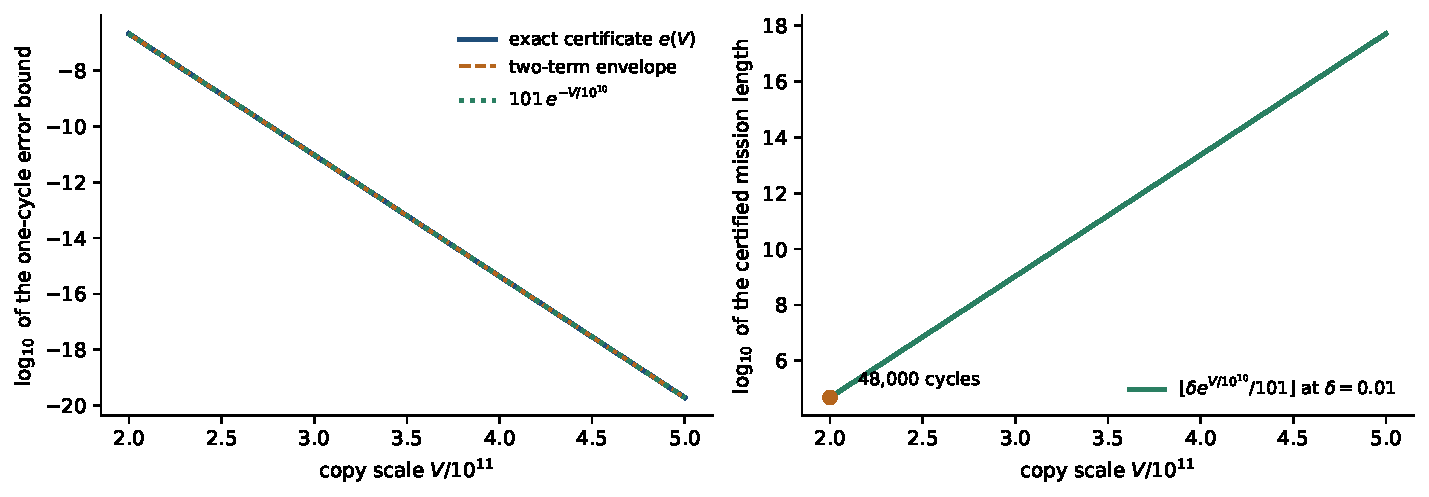
\includegraphics[width=\linewidth]{error_horizon.pdf}
\caption{Left: the exact certificate $e(V)$, the two-term envelope~\eqref{eq:envelope} and the single exponential $101e^{-V/10^{10}}$, evaluated in logarithmic form for $V\ge V_0$; the first two are visually coincident. Right: the certified mission length $\lfloor(\delta/101)e^{V/10^{10}}\rfloor$ at $\delta=0.01$. All curves are proved upper bounds, not measured failure frequencies.}
\label{fig:error}
\end{figure}

\subsection{Operating ratios}
\begin{proof}[Proof of Corollary~\ref{cor:ratios}]
On $E_m$ with $m\ge1$, $Q_I\ge m\lceil V/56\rceil>0$ and $Q_X\ge m\lceil V/1080\rceil>0$. Dividing the mission bounds of part~\ref{it:totals} by $4mV$, respectively by the output floors, gives each ratio; for instance $G/Q_I\le m\lfloor V/5\rfloor/(m\lceil V/56\rceil)\le56/5$. The demand rule combines $V_{\log}$ with $m\lceil V/56\rceil\ge D_I$ and $m\lceil V/1080\rceil\ge D_X$.
\end{proof}
Source-running time is $4m$; pulse handling and preparation are excluded. The ratios are operating allowances on one event, not optimized stoichiometric yields, and the collected output is mixed effluent.

\section{A dimensional reading}\label{sec:units}
At $V=V_0$ the hundred-cycle event has probability at least $99.9979\%$. Table~\ref{tab:counts} lists the certified counts with exact integer rounding. A richer restart witness is
\[
N_0=(186\,800\,000\,000,\ 187\,000\,000\,000,\ 12\,000\,000\,000,\ 200\,000\,000,\ 200\,000\,000,\ 200\,000\,000),
\]
with $A=B=V_0$, stock $514.6\times10^9\ge2V_0$ and $\Iv_{N_0}=12\,800\,000\,000=8V_0/125$. Its existence is separate from the reliability guarantee, which holds for every restart state.

\begin{table}[tb]
\centering\small
\begin{tabular}{lrr}
\toprule
Quantity over 100 cycles at $V=2\times10^{11}$ & Count & Approx.\ pmol\\
\midrule
Collected template equivalents & $\ge357\,142\,857\,200$ & $0.593050$\\
Collected free $X$ (included above) & $\ge18\,518\,518\,600$ & $0.0307507$\\
Each food expenditure & $\le100\,000\,000\,000\,000$ & $166.054$\\
Gross driven events & $\le4\,000\,000\,000\,000$ & $6.64216$\\
Final template inventory & $\ge7\,142\,857\,143$ & $0.0118610$\\
Net synthesis, arbitrary restart & $\ge163\,035\,714\,343$ & $0.270727$\\
Initial inventory, richer witness & $12\,800\,000\,000$ & $0.0212549$\\
Net synthesis, richer witness & $\ge351\,485\,714\,343$ & $0.583656$\\
\bottomrule
\end{tabular}
\caption{Hundred-cycle certified counts and their amount equivalents. Amounts divide the exact count by the SI Avogadro constant $N_A=6.02214076\times10^{23}\,\mathrm{mol}^{-1}$; the decimal column is descriptive and is not a sharpened inequality.}
\label{tab:counts}
\end{table}

Choose concentration and time scales $c_*,\tau_*$ and define
\begin{equation}\label{eq:units}
V=N_A\Omega c_*,\qquad t_{\rm phys}=\tau_*t,\qquad k_{\rm dim}=\frac{k_{\rm norm}}{\tau_*c_*^{\,k-1}}
\end{equation}
for a reaction of full reactant molecularity $k$; the reservoir concentrations corresponding to unit activities are $c_*$. The full driven forward reaction is bimolecular and its reverse trimolecular; substituting the maintained reservoir concentrations produces the effective propensities of Table~\ref{tab:rates}, and Appendix~\ref{app:coefficients} lists the complete conversion. Table~\ref{tab:units} gives two illustrative realizations. A change of units changes the implied physical kinetics; the examples are not calibrated protocols, and the small volume by itself establishes no feasibility claim. What the theorem could serve as is a quantitative benchmark for a maintained cell-free or synthetic reactor: preparation, supply allowances, finite-run output and confidence are specified once a matching source and handling law are justified.

\begin{table}[tb]
\centering\small
\begin{tabular}{lll}
\toprule
& $c_*=1\,\mu\mathrm M$, $\tau_*=1\,\mathrm s$ & $c_*=1\,\mathrm{mM}$, $\tau_*=60\,\mathrm s$\\
\midrule
Reactor volume $\Omega$ & $0.332108\,\mu\mathrm L$ & $0.332108\,\mathrm{nL}$\\
100-cycle source time & $400\,\mathrm s$ & $24\,000\,\mathrm s$ (6 h 40 min)\\
Bimolecular coefficient $20$ & $2\times10^{7}\,\mathrm M^{-1}\mathrm s^{-1}$ & $333.3\,\mathrm M^{-1}\mathrm s^{-1}$\\
Washout rate & $1\,\mathrm s^{-1}$ & $(1/60)\,\mathrm s^{-1}$\\
\bottomrule
\end{tabular}
\caption{Two illustrative realizations of the same normalized model at $V=2\times10^{11}$.}
\label{tab:units}
\end{table}

\section{Scope, verification boundary and open questions}\label{sec:discussion}

\paragraph{What the theorem provides.}
A finite-copy operating certificate for repeated harvesting: a restart set, a withdrawal class, a recovery schedule, output thresholds and supply allowances, and a probability bound for the joint event over any finite number of cycles, uniform over the parameter rectangle and over history-dependent controllers, together with a proof that the exported material is synthesized rather than inherited. In the language of serial transfer~\citep{mills1967,lincoln2009,adamski2020} it states the transfer fraction, the recovery time, the yield and the confidence for which the finite-molecule system is self-sustaining over a mission. In the language of continuous culture~\citep{smithwaltman1995} it is a return theorem for a pulsed stochastic chemostat with an impulsive map~\citep{lakshmikantham1989}, proved by scalar generator comparison. Relative to the companion deterministic theorem~\citep[Theorem~3.1]{recovery2026}, the four obligations it listed are discharged: the pulse is specified at the molecular level (Definition~\ref{def:intervention}); the post-pulse tails are conditional on the actual pre-pulse state (Lemmas~\ref{lem:pulsestock}--\ref{lem:pulsematerial}); return, output and supplies are proved on one continued count law with free export counted as free washout (Sections~\ref{sec:recovery}--\ref{sec:transfer}); and the conditional one-cycle bound is iterated over actual returns (Proposition~\ref{prop:product}). Its entry band~\citep[Proposition~10.1]{recovery2026} is the deterministic shadow of the prepared band and seed used here.

\paragraph{Relation to the companion stochastic certificates.}
The finite-copy exporter papers~\citep{finitecopy2026,exporter2026} certify operation from food alone over a fixed or exponential observation horizon for a reactor that is prepared once and never disturbed. The present theorem starts from established stock and certifies operation across withdrawals; the two are complementary, and the necessary initiation scale of~\citep[Theorem~6.1]{thermo2026} is the statement that governs a food-only start. The finite-count inheritance analysis~\citep{inheritance2026} concerns a different source and is not a prerequisite.

\paragraph{What is Lean-verified and what is conventional.}
Lean-verified: the twenty-label source and the identities~\eqref{eq:drift}; the pulse law, the retention factor and both pulse tails; the material corridor, exit and terminal return; guarded growth, the stock test, seeded recovery, residence; the phase comparison, the backward weights, the window bound, occupation and free collection; the template, food and service tails and their union on one law; the prepared and pulse-integrated cycle bounds; strict safety and the boundary semantics; the renewal identity, nonexplosion, the chronological semigroup and exhaustion, the literal cycle identification; the list-history process, the conditional-law model, the product bound and the full-law event; trace existence and the inventory identity; the envelope, absorption, logarithmic sizing, the fixed-scale certificates, the synthesis corollaries, the ratios and the bottleneck. Appendix~\ref{app:formal} maps each to its declaration. Conventional: the amount conversions and Table~\ref{tab:units}; the two example scales beyond $V_0$ in Table~\ref{tab:sizing}, certified by exact rational Taylor sums in the replay script; and the prose of this paper, which the Lean kernel does not check.

\paragraph{Limitations.}
Maintained activities, schematic coefficients and an ideal, conditionally independent molecular pulse are assumptions; the effective reverse driven channel has no supplied elementary implementation, and thermochemical consistency of the rate ratios does not identify molecules. Established stock must be prepared, and the first-seed result of~\citep{thermo2026} does not by itself provide the restart condition or its preparation cost. Gross driven events measure a specified chemical service; with chemical potentials a signed fuel--waste exchange supports a work calculation for that exchange, but neither is an energy bill for feed, washout, mixing, pumping, handling, preparation or purification~\citep{rao2016,rao2018}. Output is mixed effluent. The theorem certifies finite missions at a chosen scale, not eternal survival at one volume, food-only startup, autonomous operation with finite baths, a causal knockout comparison or the performance of any named biochemical system.

\paragraph{Open questions.}
Four seem most natural. First, the phase bottleneck: the certificate's scale is set entirely by the term $100e^{-V/10^{10}}$ of the occupation estimate, whose tilt $10^{-6}$ is forced by the quadratic remainder of the phase test over $91V$ clock steps; a sharper transport estimate, for instance with a state-dependent tilt or a two-window argument, would lower $V_0$ by orders of magnitude, whereas recovery contributes only $e^{-3V/5\cdot10^6}$. Second, a large-deviation form of the same question~\citep{agazzi2018}: the present constants are sufficient, not sharp, and no rate function is claimed. Third, feedback: whether a controller acting on the returned history can be chosen to maximize certified yield per unit of food or service, a stochastic control problem on the history chain. Fourth, food-only startup with a subsequent switch to the harvesting protocol, which would join the initiation certificate of~\citep{thermo2026} to the present restart set through an explicit preparation cycle.

\paragraph{Data and code availability.}
\RepositoryNote{} The Lean sources, the strict verification receipts, the figure script and an exact replay script for every printed constant accompany the manuscript source.

\appendix
\section{Complete error budget}\label{app:error}
For $V\ge0$ define
\begin{align*}
M(V)&=4e^{-V/2000}+48000V\,e^{-V/2000+1/50},\\
R(V)&=e^{-3V/5000000}+e^{-V/2}+M(V)+e^{-V/10000}+12000V\,e^{-V/10000+9/500},\\
F(V)&=e^{-V/40000000}+100e^{-V/10000000000}+e^{-V}+e^{-V/200},\\
J(V)&=F(V)+e^{-V/100000}+2e^{-V/300}+e^{-V/2000},\\
T(V)&=M(V)+R(V)+4\bigl(e^{-V/320000}+e^{-V}\bigr),\\
e(V)&=e^{-1177V/1000000000}+4e^{-V/100000}+J(V)+T(V).
\end{align*}
This is exactly the source's \lean{oneCycleError}; repeated material terms are retained rather than optimized away. $J$ is the joint five-counter budget and $T$ the restart budget; the two pulse terms are outside the prepared-cycle budget. Figure~\ref{fig:residual} shows the residual of the two-term envelope in logarithmic form; values far below floating-point range remain finite logarithms and are never interpreted as zero.

\begin{figure}[tb]
\centering
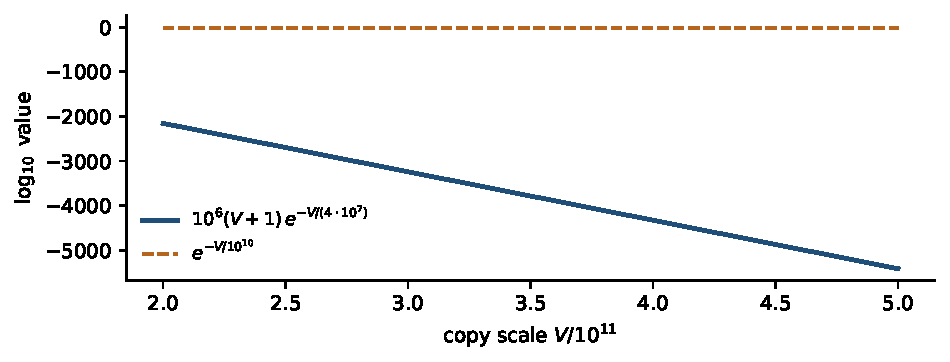
\includegraphics[width=0.72\linewidth]{residual.pdf}
\caption{The polynomial-exponential residual of the envelope~\eqref{eq:envelope} against the phase term, for $V\ge V_0$. Lemma~\ref{lem:absorb} proves the ordering exactly by a sixth-order Taylor comparison.}
\label{fig:residual}
\end{figure}

\section{Quantitative exponential tests}\label{app:tests}
This appendix records the inequalities underlying the cycle estimates so that the probabilistic argument can be read without the implementation modules.

\paragraph{Elementary inequalities.}
For $|z|\le9/50$, $e^z\le1+z+\tfrac35z^2$. For $0\le x$, $e^x\ge\sum_{k\le n}x^k/k!$. For $0<a<1$, $\log a\ge1-1/a$. For a Poisson variable of mean $\mu$ and $k<\mu$, $\Prob(\Poi(\mu)\le k)\le e^{-(\mu-k)^2/(2\mu)}$~\citep{chernoff1952}.

\paragraph{Pulse.}
With independent Bernoulli indicators $B_a$ of parameters $p_a$ and weights $w_a\ge0$, $\E\exp(s\sum_aw_aB_a)=\prod_a(1-p_a+p_ae^{sw_a})$ exactly. Stock weights are at most $9/5$ and Lemma~\ref{lem:factor} applies at $s=1/100$ with $\sum p_aw_a\ge49V/4000$ and level $3V/250$, giving $-1177V/10^9$. Material weights are at most $2$; the unrounded post-pulse material means lie in $[31213V/32000,\,3231V/3200]$ and the floor lowers a mean by less than one, leaving the slack required for $[24V/25,\,51V/50]$ at $V\ge10^6$; the bounded-weight exponential estimate gives $e^{-V/100000}$ per sign and coordinate.

\paragraph{Material barriers and terminal return.}
For $H\in\{A,B\}$ the barriers $U_H=e^{(H-11V/10)/100}$ and $L_H=e^{-(H-9V/10)/100}$ sum to at least one on exit and to at most $4e^{-V/2000}$ over both coordinates at a prepared start; on the corridor each has generator at most $3000Ve^{-V/2000+1/50}$, since outside the inner band $|H-V|\le V/20$ the restoring drift dominates and inside it a jump of size at most $2$ shifts the exponent by at most $1/50$. Integration over four units gives $M(V)$. For terminal return the compensated tilt $e^{-2s^2V}T_s$ contracts its parameter by $1-1/(3000V)$ per step; $n\ge11700V$ gives a factor at most $1/40$; $s=\pm1/1000$ and $|H_0-V|\le V/25$ give exponent at most $-V/320000$ for $|H-V|\ge V/160$; the clock of mean $12000V$ misses $11700V$ with probability at most $e^{-V}$.

\paragraph{Seeded recovery and residence.}
Below $3V/50$ the drift is at least $\tfrac23Y+V/10^9$ and the rate-weighted squared stock jumps are at most $6Y+V/10^8$, so $\Lgen e^{-sY}\le-\tfrac58sYe^{-sY}$ for $s\le1/100$. The killed entry test satisfies $PT_s\le T_t$ for $t\le(1+\tfrac{5/8}{3000V})s$; starting at $1/1000$ and capping at $101/20000$, the block estimate $(1+\tfrac{5/8}{3000V})^{8100V}\ge(17/16)^{27}>101/20$ shows the cap is reached; the exponential Markov inequality gives $\exp\{\tfrac1{1000}\cdot\tfrac{3V}{50}-\tfrac{101}{20000}\cdot\tfrac{3V}{250}\}=e^{-3V/5000000}$; the clock of mean $8250V$ misses $8100V$ with probability at most $e^{-V/2}$. Residence uses $H_Y=\max(e^{-Y/100},e^{-3V/5000})$ with generator at most $3000Ve^{-3V/5000+9/500}$, worth $e^{-V/2000}$ at a lower exit and $e^{-3V/5000}$ at the start; integration over $t\le4$ gives $e^{-V/10000}+12000Ve^{-V/10000+9/500}$.

\paragraph{Phase margin and collection tilt.}
In~\eqref{eq:weights}, $a^n\ge1/12$ for $n\le91V$, and $n\ge89V$, $n-1\ge88V$ give each coordinate at least $1/35$ of its stock weight. The remainder per step is $\tfrac{12}5s^2$; at $s=10^{-6}$ the total over $91V$ steps is at most $\tfrac{12}5\cdot91V\cdot10^{-12}$. The threshold $N_X\le V/1000$ contributes $V/10^9$ and the initial stock $-V/(700\cdot10^6)$; the sum is at most $-V/10^{10}$. After a burn-in of $90V$ steps this bounds low-free occupancy at every later step; with $B$ the number of bad steps among $n$, $\E B\le ne^{-V/10^{10}}$ and $\Prob(B\ge n/100)\le100e^{-V/10^{10}}$. The marked tilt of size $1/1000$ on $Q_X+B/(3\cdot10^6)$ gives $\exp\{\tfrac1{1000}(K+\tfrac{B_*}{3\cdot10^6})-\tfrac{33n}{10^{11}}\}+\Prob(B\ge B_*)$ with $K=V/1080+1$, $B_*=n/100$, $n\ge2990V$; for $V\ge10^6$ the first term is at most $e^{-V/40000000}$. The precollection quarter unit and the collection unit have clock means $750V$ and $3000V$, contributing $e^{-V}$ and $e^{-V/200}$.

\paragraph{Template and supply arithmetic.}
For a nonnegative mark bounded by $2$, the one-step lower-tail test at tilt $1/1000$ is controlled by the mean mark; template washout has mean mark at least $1/84000$ per active step, hence multiplier at most $e^{-33/2800000000}$, and Poisson summation with mean $3000V$ gives $\tfrac{V/56+1}{1000}+3000V(e^{-33/2800000000}-1)\le-V/100000$ for $V\ge10^6$. For a supply with rate at most $cV$, initial count $z$ and threshold $K$ the upper-tail exponent is $-sK+4cV(e^s-1)+sz$: $c=1$, $s=1/50$, $z\le151V/200$, $K=5V$ give at most $-V/300$; $c=9/200$, $s=1/20$, $z=0$, $K=V/5-1$ give at most $-V/2000$ for $V\ge10^6$.

\section{Complete dimensional coefficients}\label{app:coefficients}
Table~\ref{tab:coefficients} gives the full chemical rate coefficients under~\eqref{eq:units}. A coefficient for molecularity $k$ has units $\mathrm M^{1-k}\mathrm s^{-1}$. The effective pair-5 coefficients after substituting $[F]=[P]=c_*$ are $d/\tau_*$ (unimolecular forward) and $d\eta/(\tau_*c_*)$ (bimolecular reverse); they must not be confused with the full chemical coefficients. Either food feed becomes a concentration input $c_*/\tau_*$ and a molecular arrival rate $V/\tau_*$; every washout coefficient is $1/\tau_*$; the pulse food counts and retention probabilities remain dimensionless. Preparation and handling durations lie outside the four-unit source interval.

\begin{table}[tb]
\centering\small
\begin{tabular}{clcc}
\toprule
Pair & Directional molecularities & $k^+_{\rm dim}$ & $k^-_{\rm dim}$\\
\midrule
0 & $2,1$ & $\eps/(\tau_*c_*)$ & $\eps/(10\tau_*)$\\
1 & $2,1$ & $20/(\tau_*c_*)$ & $20/\tau_*$\\
2 & $2,1$ & $20/(\tau_*c_*)$ & $20/\tau_*$\\
3 & $1,1$ & $20/\tau_*$ & $2/\tau_*$\\
4 & $1,2$ & $r/\tau_*$ & $r/(\tau_*c_*)$\\
5 & $2,3$ & $d/(\tau_*c_*)$ & $d\eta/(\tau_*c_*^2)$\\
\bottomrule
\end{tabular}
\caption{Normalized and dimensional full-reaction coefficients.}
\label{tab:coefficients}
\end{table}

\section{Formal evidence and reproduction}\label{app:formal}
The frozen environment is Lean~4 (toolchain \lean{leanprover/lean4:v4.30.0}) with the repository's pinned Mathlib manifest. Verification treats compiler warnings as errors, exports declaration types and reports the axioms used. All declarations live in the namespace \lean{FiniteCopyReactor} under \lean{proofs/FiniteCopyReactor/}; the count source is bound to the realization of~\citep{thermo2026} through \lean{CommonPhysicalRealization.ExporterSource}. The original root \lean{Resolution.lean} exports \lean{finite_copy_reactor_horizon} (the full-law event with the linear bound), \lean{finite_copy_reactor_result} (the earlier linear sizing with an explicit restart witness), \lean{finite_copy_reactor_hundred} and \lean{finite_copy_reactor_adapted_history}. The publication root \lean{PublicationResolution.lean} adds \lean{publication_logarithmic}, \lean{publication_48000}, \lean{publication_hundred} and \lean{certified_mission_budget}, and its strict receipt authenticates six interfaces: these three together with \lean{full_operational_product}, \lean{HistoryTrace.sharp_uniform_integer} and \lean{operational_ratios}. Each depends only on the standard axioms \lean{propext}, \lean{Classical.choice} and \lean{Quot.sound}; there are no admitted placeholders, no custom axioms and no warning suppression. The publication receipt records exit code $0$, empty compiler output, $238$ current local dependency sources and a source SHA-256 beginning \lean{bc121e4a}; the original root receipt has $234$ dependency sources and root SHA-256 beginning \lean{6ec29251}.

The compiled event \lean{OperationalSuccess N V m policy} is the set of histories of length $m$ whose every record satisfies Definition~\ref{def:success}, for which a physical trace exists, whose five totals satisfy the bounds of part~\ref{it:totals}, and whose every trace satisfies the real form of~\eqref{eq:sharp}; \lean{full_operational_product} bounds its probability under the $m$-step list-history kernel from the empty list by $(1-e(V))^m$, and \lean{physical_history_product} does the same for every structure \lean{PhysicalHistory} satisfying the conditional-law and actual-return fields. The intervention structure carries the bounds~\eqref{eq:pulsebounds} as proof obligations, and the parameter hypotheses are $19\le r\le21$ and $0\le d\le1/25$ in the stochastic chain, $1/50\le d$ at the publication interfaces.

\begin{longtable}{>{\raggedright\arraybackslash}p{0.36\linewidth}>{\raggedright\arraybackslash}p{0.58\linewidth}}
\toprule Claim & Principal declarations or modules\\\midrule\endhead
\bottomrule\endlastfoot
Literal twenty-label source and identities~\eqref{eq:drift} (Section~\ref{sec:source}) & \lean{Source}: \lean{material_A_generator}, \lean{material_B_generator}, \lean{stock_generator_correction}, \lean{count_guarded_growth}; \lean{JointCountSource}\\
Restart set and witnesses (Definition~\ref{def:restart}) & \lean{Restart}: \lean{restart_witness}, \lean{restart_nonempty}; \lean{all_free_restart}\\
Molecular pulse law, retention factor, stock tail (Lemmas~\ref{lem:factor}, \ref{lem:pulsestock}) & \lean{Pulse}: \lean{pulseMass_total}, \lean{pulse_laplace}, \lean{retention_factor_bound}, \lean{pulse_chernoff}; \lean{PulseStock}; \lean{PulseInventory}\\
Pulse material tails and doses (Lemma~\ref{lem:pulsematerial}) & \lean{PulseMaterial}, \lean{PulseMaterialProbability}, \lean{PulseDeviation}, \lean{pulse_food_budget}\\
Corridor, uniformization, exit, terminal return (Lemmas~\ref{lem:corridor}, \ref{lem:terminal}) & \lean{MaterialModel}, \lean{MaterialPulse}, \lean{MaterialReturn}, \lean{TerminalMaterial}, \lean{TerminalMaterialProbability}, \lean{SwitchedMaterial}\\
Stock test and seeded recovery (Lemma~\ref{lem:stocktest}, Proposition~\ref{prop:entry}) & \lean{StockExponential}, \lean{EntrySchedule}, \lean{EntryProbability}: \lean{seeded_recovery_deadline}\\
Residence and actual continuation (Lemma~\ref{lem:residence}) & \lean{ResidencePotential}, \lean{Residence}, \lean{ClampedResidence}, \lean{CollectionResidence}, \lean{DeadlineStock}\\
Phase drifts, weights, window (Lemmas~\ref{lem:phase}, \ref{lem:weights}, Proposition~\ref{prop:lowfree}) & \lean{PhaseComparison}, \lean{PhaseWeights}, \lean{PhaseWindow}, \lean{PhaseTime}, \lean{PhaseProbability}: \lean{phase_discrete_probability}\\
Occupation and free collection (Proposition~\ref{prop:free}) & \lean{Occupation}: \lean{occupation_after_burnin}, \lean{bad_occupation_bound}; \lean{FreeCollection}: \lean{free_collection_probability}; \lean{FreeThreshold}\\
Template, food, service tails (Lemmas~\ref{lem:template}, \ref{lem:supply}) & \lean{Template}, \lean{TemplateThreshold}, \lean{SupplyBudget}, \lean{SupplySource}, \lean{RoundedService}, \lean{MarkedUpper}\\
Joint counter budget on one law (Proposition~\ref{prop:counters}) & \lean{JointMarks}, \lean{JointCycle}, \lean{JointTails}, \lean{JointSupplyTails}, \lean{JointCounterBudget}: \lean{joint_counter_budget}\\
Prepared and pulse-integrated cycle (Propositions~\ref{prop:prepared}, \ref{prop:stopped}) & \lean{PreparedCycle}, \lean{StateRestart}, \lean{PulseCycle}: \lean{pulse_cycle_failure_bound}, \lean{oneCycleError}\\
Strict safety and boundary semantics (Lemma~\ref{lem:strict}, Remark~\ref{rem:boundary}) & \lean{SafeCycle}, \lean{StoppingSemantics}, \lean{CountCycleEvent}\\
Renewal identity and killed comparison (Lemma~\ref{lem:renewal}) & \lean{StoppedAgreement}: \lean{stopped_clock_eq_killed_chronology}, \lean{stopped_clock_le_unrestricted}; \lean{KilledChronology}, \lean{SurvivalResolvent}, \lean{ScalarRenewal}\\
Nonexplosion (Lemma~\ref{lem:nonexplosion}) & \lean{CountNonexplosion}, \lean{JointTrajectory}: \lean{joint_trajectory_nonexplosion}; \lean{ActualSource}\\
Chronological semigroup, exhaustion, literal cycle law (Proposition~\ref{prop:semigroup}) & \lean{SourceSemigroup}: \lean{chronological_endpoint_semigroup}; \lean{JointTimeComposition}: \lean{joint_source_cycle_kernel_literal}; \lean{JointPhysicalEndpoint}\\
One cycle on the physical law (Theorem~\ref{thm:onecycle}) & \lean{LiteralCycleBound}: \lean{literal_cycle_success_bound}\\
History process and product bound (Definition~\ref{def:process}, Proposition~\ref{prop:product}) & \lean{ReturnedHistory}, \lean{PhysicalHistory}, \lean{HistorySurvival}, \lean{HistoryFullLaw}, \lean{OperationalCorollaries}: \lean{physical_history_product}, \lean{full_operational_product}\\
Trace existence and inventory (Lemma~\ref{lem:inventory}, Proposition~\ref{prop:synthesis}) & \lean{PhysicalHistoryInventory}: \lean{full_history_has_trace}, \lean{HistoryTrace.inventory_lower}; \lean{SynthesisCorollaries}: \lean{restart_final_inventory}, \lean{HistoryTrace.sharp_uniform_integer}, \lean{HistoryTrace.positive_after_55}, \lean{HistoryTrace.rich_two_cycle}, \lean{HistoryTrace.hundred_uniform_integer}, \lean{HistoryTrace.hundred_rich_integer}\\
Envelope, absorption, sizing (Lemmas~\ref{lem:envelope}, \ref{lem:absorb}, Corollary~\ref{cor:scale}) & \lean{ErrorEnvelope}: \lean{one_cycle_error_envelope}; \lean{LogarithmicScale}: \lean{residual_error_absorbed}, \lean{one_cycle_single_exponential}, \lean{logarithmic_volume_error}, \lean{exp_twenty_certificate}, \lean{mission_48000_budget}, \lean{hundred_sharp_budget}; \lean{PublicationResolution}\\
Earlier linear rule (Remark~\ref{rem:linear}) & \lean{EffectiveScale}: \lean{volume_times_error}, \lean{sufficient_volume_error}; \lean{finite_copy_reactor_result}\\
Ratios (Corollary~\ref{cor:ratios}) & \lean{operational_ratios}\\
Bottleneck (Proposition~\ref{prop:bottleneck}) & \lean{ErrorBottleneck}: \lean{one_cycle_error_phase_lower}, \lean{error_certificate_volume_limit}\\
Theorem~\ref{thm:main}, all parts & \lean{finite_copy_reactor_horizon}; \lean{full_operational_product}; \lean{publication_budget}\\
\end{longtable}

\paragraph{Reproduction.}
From the repository root, with the canonical interpreter and the pinned wrapper (one command per line, continuation lines joined):
\begin{quote}\small\ttfamily\raggedright
.\textbackslash.venv\textbackslash Scripts\textbackslash python.exe scripts/check\_python.py --quiet\par
.\textbackslash.venv\textbackslash Scripts\textbackslash python.exe scripts/verify\_proof.py proofs/FiniteCopyReactor/PublicationResolution.lean\par
\quad --declaration FiniteCopyReactor.publication\_logarithmic\par
\quad --declaration FiniteCopyReactor.publication\_48000\par
\quad --declaration FiniteCopyReactor.publication\_hundred\par
\quad --declaration FiniteCopyReactor.full\_operational\_product\par
\quad --declaration FiniteCopyReactor.HistoryTrace.sharp\_uniform\_integer\par
\quad --declaration FiniteCopyReactor.operational\_ratios\par
\quad --output [workspace]/PublicationResolution.verify.json
\end{quote}
Here \lean{[workspace]} is the campaign folder that holds the receipts. The wrapper runs Lean serially in the pinned \lean{mathlib4_project} directory with warnings as errors; no dependency update is required. The script \lean{check_paper.py} accompanying this source replays every constant printed above ($132$ checks: exact generator identities, pulse means and exponents, corridor rates, tilt schedules, phase weights, counter exponents, the envelope, the Taylor certificates, the counts, the ratios and the unit conversions) and \lean{make_figures.py} regenerates the figures from the proved bounds.

\bibliographystyle{plainnat}
{\small\bibliography{refs}}

\end{document}
